%!TEX root = ../report.tex

\begin{document}
    \chapter{Experimental Evaluation}
\section{Metrics}
\subsection{Kullback-Leiber Divergence}\label{sec_kl_div}
\subsection{Root Mean Squared Error(RMSE)}
Root Mean Squared Error (RMSE), measures the spread of distances between model predictions and their corresponding ground truth values. Alternatively, it can be explained as the standard deviation of prediction errors. RMSE is a well-known accuracy metric in regression problems. The metric is non-negative in nature with lower values indicating better model fit.
\begin{equation}
	\mathbf{RMSE} = \sqrt{\frac{\sum_{i=1}^{N}(\hat{y}_i-y_i)^2}{N}}
\end{equation}
Here $\hat{y}$,$y$ and $N$ represent ground truth labels, predictions and number of data points respectively.
\subsection{Explained Variance(EVA)}
The Explained Variance (EVA) is a measure of a regressor's ability to capture variance(variation) of given data. The metric can be computed with the following expression:
\begin{equation}
	\mathbf{EVA} = \frac{Variance(\hat{y}-y)}{Variance(\hat{y})}
\end{equation}
Here $\hat{y}$,$y$ represent ground-truth labels and predictions respectively. The numerator term denotes variance of residuals whereas the denominator denotes the underlying variance in ground-truth labels. For an ideal regressor, the value of EVA equals 0.
\subsection{Negative-Log-Likelihood(NLL)}
In this research work,the Negative-Log-Likelihood(NLL) metric is used compare performance of uncertainty estimation methods. NLL for a given pair of prediction and uncertainty can be computed as follows
\begin{itemize}
	\item A distribution (often Gaussian) is created with the model prediction as its mean and uncertainty as its variance.
	\item The conditional probability of observing the ground-truth label(corresponding to the input) in the created distribution is determined. This is nothing but the likelihood value of ground-truth in the created distribution.
	\item  In order to handle and effectively represent very low values of likelihood, negative of natural logarithm is applied  to the value. After application of negative logarithm, the total likelihood can be computed by summing all individual values.
\end{itemize}
\begin{equation}
	\mathbf{NLL} = -\sum_{i=1}^{N}\ln P(\hat{y}_i|\mathcal{N}(y_i,\sigma^2)) 
\end{equation}
Here $\hat{y}$,$y$,$\sigma^2$ and $N$ represent ground truth labels, predictions, predictive uncertainty and number of data points respectively.
Lower the value of NLL better the performance of an uncertainty estimation method associated with it. However, the value of NLL highly depends on the number and choice of test points used for evaluation. Therefore, the metric can be used to compare performance of uncertainty estimation methods only when the same data set is used for their evaluation.
\subsubsection{Limitations of NLL}
NLL measures the goodness of fit of the approximated posterior distribution to the true function's mean(ground truth). The metric fails to evaluate fidelity of the approximated posterior distribution. Therefore, NLL "may be a good criteria for model
selection, it is not a reliable criteria for determining how well an approximate posterior aligns with the true posterior"\cite{yao2019quality}. This can be understood better with help of the illustration below.  

\section{Predictive accuracy and uncertainty quality}
\subsection{Quantitative comparison}
\begin{table}[h!]
	\centering
	\begin{tabular}{|c|c|c|c|c|c|}
		\hline
		\multirow{2}{*}{\textbf{Model}} & \multirow{2}{*}{\textbf{RMSE}} & \multirow{2}{*}{\textbf{EVA}} & \multicolumn{3}{c|}{\textbf{NLL}}                             \\ \cline{4-6} 
		&                                &                               & \textbf{Epistemic} & \textbf{Aleatoric} & \textbf{Predictive} \\ \hline
		Vanilla Dronet                  & 0.034                          & 0.98                          & NA                 & NA                 & NA                  \\ \hline
		MCDO\_ADF Dronet                & 0.15                           & 0.68                          & -0.71              & 7.51               & -0.74               \\ \hline
		Evidential Dronet               & \textbf{0.022}                 & \textbf{0.99}                 & \textbf{-2.03}     & \textbf{-1}        & \textbf{-0.94}      \\ \hline
	\end{tabular}
	\caption{A quantitative comparison of uncertainty estimation methods when applied to Dronet}
	\label{tab_quant_compare}
\end{table}
\begin{itemize}
	\item It can be inferred that Evidential Dronet outperforms the other two models in terms of both predictive accuracy and quality of uncertainty estimation.
	\item In the case of predictive accuracy expressed in terms of RMSE, Evidential Dronet outperforms the Vanilla variant only by a slight margin. However, difference in RMSE between Evidential and MCDO\_ADF variants is considerable. This could be partly attributed to the fact that both predictions and uncertainty estimates outputted by the MCDO\_ADF variant depend on the count of Monte-Carlo(MC) samples considered. Higher the value of MC samples better the model's performance(refer figure \ref{fig_mc_count_vs_rmse}).  However, this holds true only un till a particular value of MC samples. For this experiment, 20 MC samples are considered. 
	\item The relationship between MC sample counts and predictive accuracy holds good for the Explained Variance (EVA) measure as well.
	\item The quality of predictive uncertainty estimated by the Evidential Dronet expressed in terms of Negative-Log-Likelihood (NLL) is better than the MCDO\_ADF variant. This intuitively means that the former technique is able to determine parameters of the distribution in which likelihood of finding ground truth labels is higher than in the distribution outputted by the latter.
\end{itemize}
\begin{figure}[h]
	\centering
	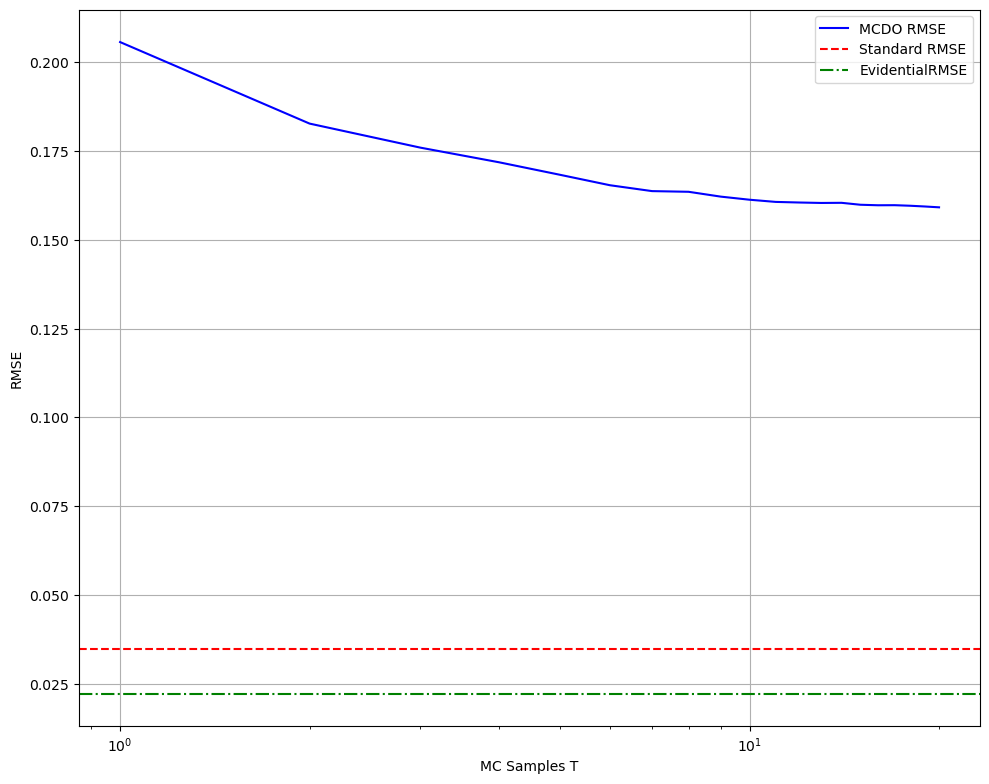
\includegraphics[scale=0.5]{RMSE_T20}
	\caption{A plot depicting relationship between the MC sample count and RMSE during the MCDO\_ADF model inference}
	\label{fig_mc_count_vs_rmse}
\end{figure}
\subsection{Qualitative comparison}
In order to qualitatively compare predictive uncertainties outputted by both the models, test images corresponding to the highest and lowest values of uncertainty(aleatoric, epistemic and predictive) are taken into consideration and analyzed. The analysis is presented in the table below.
\begin{table}[h!]
\flushleft
\begin{tabular}[ht]{|p{1.5cm}|p{2.3cm}|p{13.8cm}|}
\hline
\textbf{Category}&\textbf{Method}&\textbf{Analysis}\\
\hline
Aleatoric&MCDO\_ADF&\begin{itemize}\item The method performs well in estimating data uncertainty.The presence of glare, blur, and poor illumination in images reported with high values show that the estimated uncertainty is indeed aleatoric. \item Most of the images reported with low values of aleatoric uncertainty are characterized by high contrast and low noise levels. \item There also exist certain over-illuminated images for which the method reports a low value of data-uncertainty and is undesirable.\end{itemize}\\
\hline
Aleatoric&DER/Evidential&\begin{itemize}\item The method reports a high-value of aleatoric uncertainty for blurry and unclear images and is desirable.\item  It is interesting to note that this method reports high-values of data uncertainty for images with objects such as grass that produce patterns similar to noise.\item Similar to MCDO\_ADF this method performs well in reporting low aleatoric uncertainty for clear images except for the ones with shadows.\end{itemize}\\
\hline
Epistemic&MCDO\_ADF&\begin{itemize}\item The method reports high values of epistemic uncertainty for both images with unclear lane markings(intuitively a key feature to predict steering angles) and noise induced by factors such as blur and glare.\item Reporting high values of epistemic uncertainty for noisy images proves the method's ability to jointly model both the components of uncertainty.\item Similar to the aleatoric case, the method reports low values of epistemic uncertainty for clear images except for the ones with poor and over illumination.\end{itemize}\\
\hline
Epistemic&DER/Evidential&\begin{itemize}\item The method produces high values of model uncertainty for both images with unclear features and noise, similar to MCDO\_ADF.\item However, there is a difference between images reported with high values of epistemic uncertainty between MCDO\_ADF and evidential showing the fact that they both have different criteria for uncertainty estimation.\item The set of images reported with low values of epistemic uncertainty have a lot of similarities with that of ones with low-aleatoric variances.\end{itemize}\\
\hline
Total& MCDO\_ADF and DER/Evidential&\begin{itemize}\item The set of images reported with high/low values of predictive uncertainties by both the methods correspond to the ones with high/low values of their components(aleatoric and epistemic).\item This could be attributed to the fact that the predictive uncertainty is obtained as the sum of its components in both the methods.\end{itemize}\\
\hline

\end{tabular}
\caption{A qualitative comparison of uncertainty estimation methods when applied to Dronet}
\label{tab_qualit_compare}
\end{table}

\end{document}
\section{Out-Of-Distribution(OOD) testing}
One of the important uses for having an estimate of uncertainty associated with a Neural Net model's output is "selective prediction". This means that the confidence estimate can be used to determine the correctness of an output and in turn decide whether to consider it for further processing/decision-making or not. It is crucial for the uncertainty estimation method to produce a higher value of uncertainty when the model faces test samples from an unknown data distribution. This section evaluates the considered uncertainty estimation methods on their response to out-of-distribution inputs.
\subsection {Response to Out-Of-Distribution data}
\subsection{Robustness to adversarial attacks}
Adversarial examples are malicious inputs designed to fool machine learning models[\cite{kurakin2016adversarial}]. Such data samples can be considered as an extreme case of Out-Of-Distribution as they are synthesized by perturbing inputs in an adversarial fashion to cause maximum error on the model prediction. An uncertainty estimation method needs to be capable of identifying and reporting an adversarially perturbed input data sample by producing a high value of uncertainty. 

In order to evaluate the robustness of the considered uncertainty estimation methods, samples from training data distribution are perturbed using the FGSM(Fast Gradient Sign Method)\cite{goodfellow2015explaining} and fed to the trained ResNet-8 model. Changes in the estimated values of predictive uncertainty and RMSE with respect to increasing levels of perturbation(denoted by $\epsilon$) between 0 and 0.1 for a given image are plotted in the graphs shown in the figure\ref{fig_adv_analysis_single}. A set of images produced from a given image subject to different levels of adversarial perturbations is shown in the figure\ref{fig_adv_example}.

\begin{figure}[h]
	\centering
	\begin{subfigure}[b]{0.19\textwidth}
		\centering
		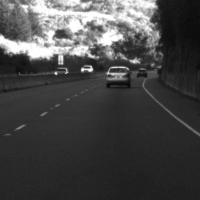
\includegraphics[width=\textwidth]{adv_0}
		\caption{$\epsilon=0$}
		\label{fig:y equals x}
	\end{subfigure}
	\hfill
	\begin{subfigure}[b]{0.19\textwidth}
		\centering
		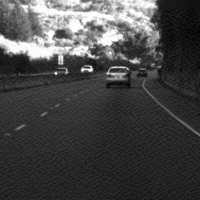
\includegraphics[width=\textwidth]{adv_1}
		\caption{$\epsilon=0.02$}
		\label{fig:three sin x}
	\end{subfigure}
	\hfill
	\begin{subfigure}[b]{0.19\textwidth}
		\centering
		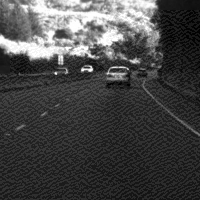
\includegraphics[width=\textwidth]{adv_2}
		\caption{$\epsilon=0.06$}
		\label{fig:five over x}
	\end{subfigure}
	\hfill
	\begin{subfigure}[b]{0.19\textwidth}
		\centering
		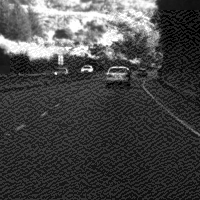
\includegraphics[width=\textwidth]{adv_3}
		\caption{$\epsilon=0.08$}
		\label{fig:five over x}
	\end{subfigure}
	\hfill
	\begin{subfigure}[b]{0.19\textwidth}
		\centering
		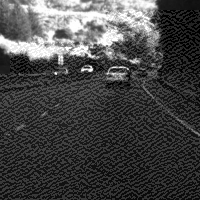
\includegraphics[width=\textwidth]{adv_4}
		\caption{$\epsilon=0.10$}
		\label{fig:five over x}
	\end{subfigure}
	\caption{Images depicting increasing levels of Adversarial noise}
	\label{fig_adv_example}
\end{figure}

\begin{figure}[h]
	\centering
	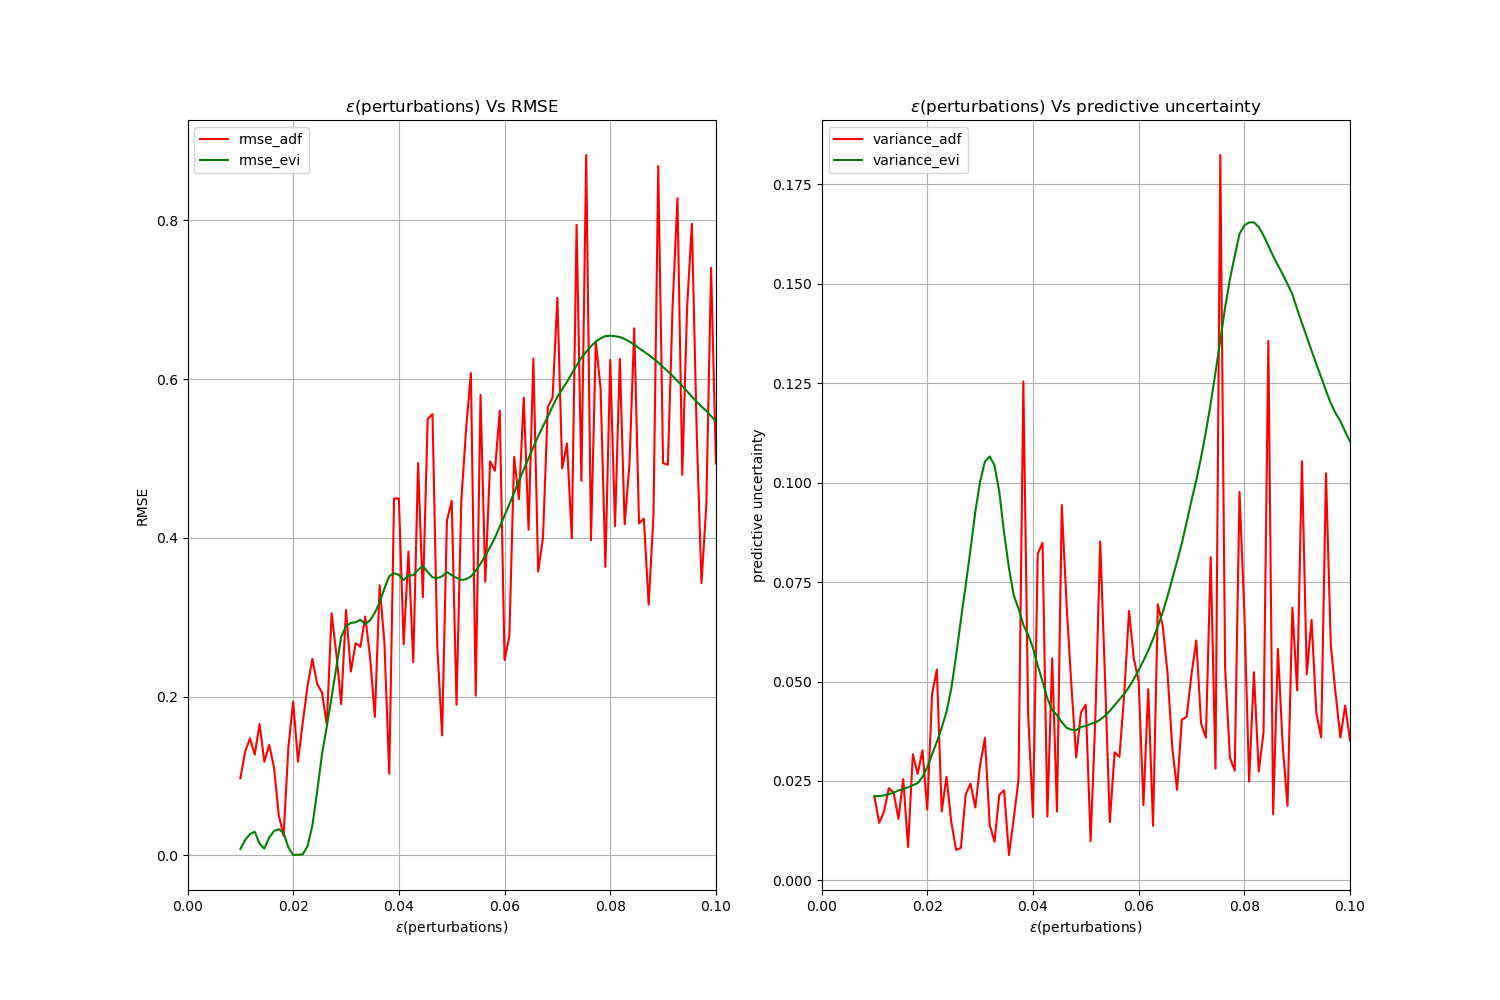
\includegraphics[scale=0.40]{adversarial_analysis_single}
	\caption{(a) Plot depicting the change in RMSE with respect to increase in adversarial perturbations for a single image (b) Plot depicting the change in predictive uncertainty with respect to increase in adversarial perturbations for a single image}
	\label{fig_adv_analysis_single}
\end{figure}



It can be inferred from the plot that the increase in values of RMSE of the model using DER is consistent with the increase in perturbation levels, while a lot of variations can be observed in the case of MCDO\_ADF variant. In the case of relationship between $\epsilon$ and predictive uncertainty, the predictive uncertainties estimated by DER remains almost constant in the interval between $\epsilon = $ but increase steadily then after. Similar to the case of $\epsilon$ Vs RMSE, a lot of fluctuations can be observed in the uncertainty estimates produced for different levels of $\epsilon$.

\begin{figure}[h]
	\centering
	\begin{subfigure}[b]{0.4\textwidth}
	\centering
	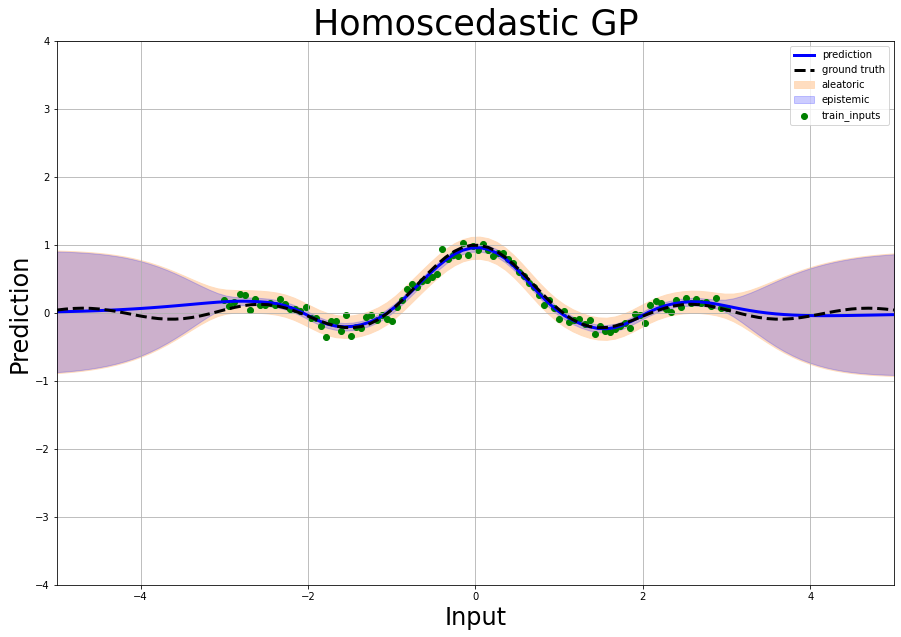
\includegraphics[width=\textwidth]{toy_dataset/homo_fn1}
	\caption{$\epsilon=0$}
	\label{fig:y equals x}
	\end{subfigure}
	\hfill
	\begin{subfigure}[b]{0.4\textwidth}
	\centering
	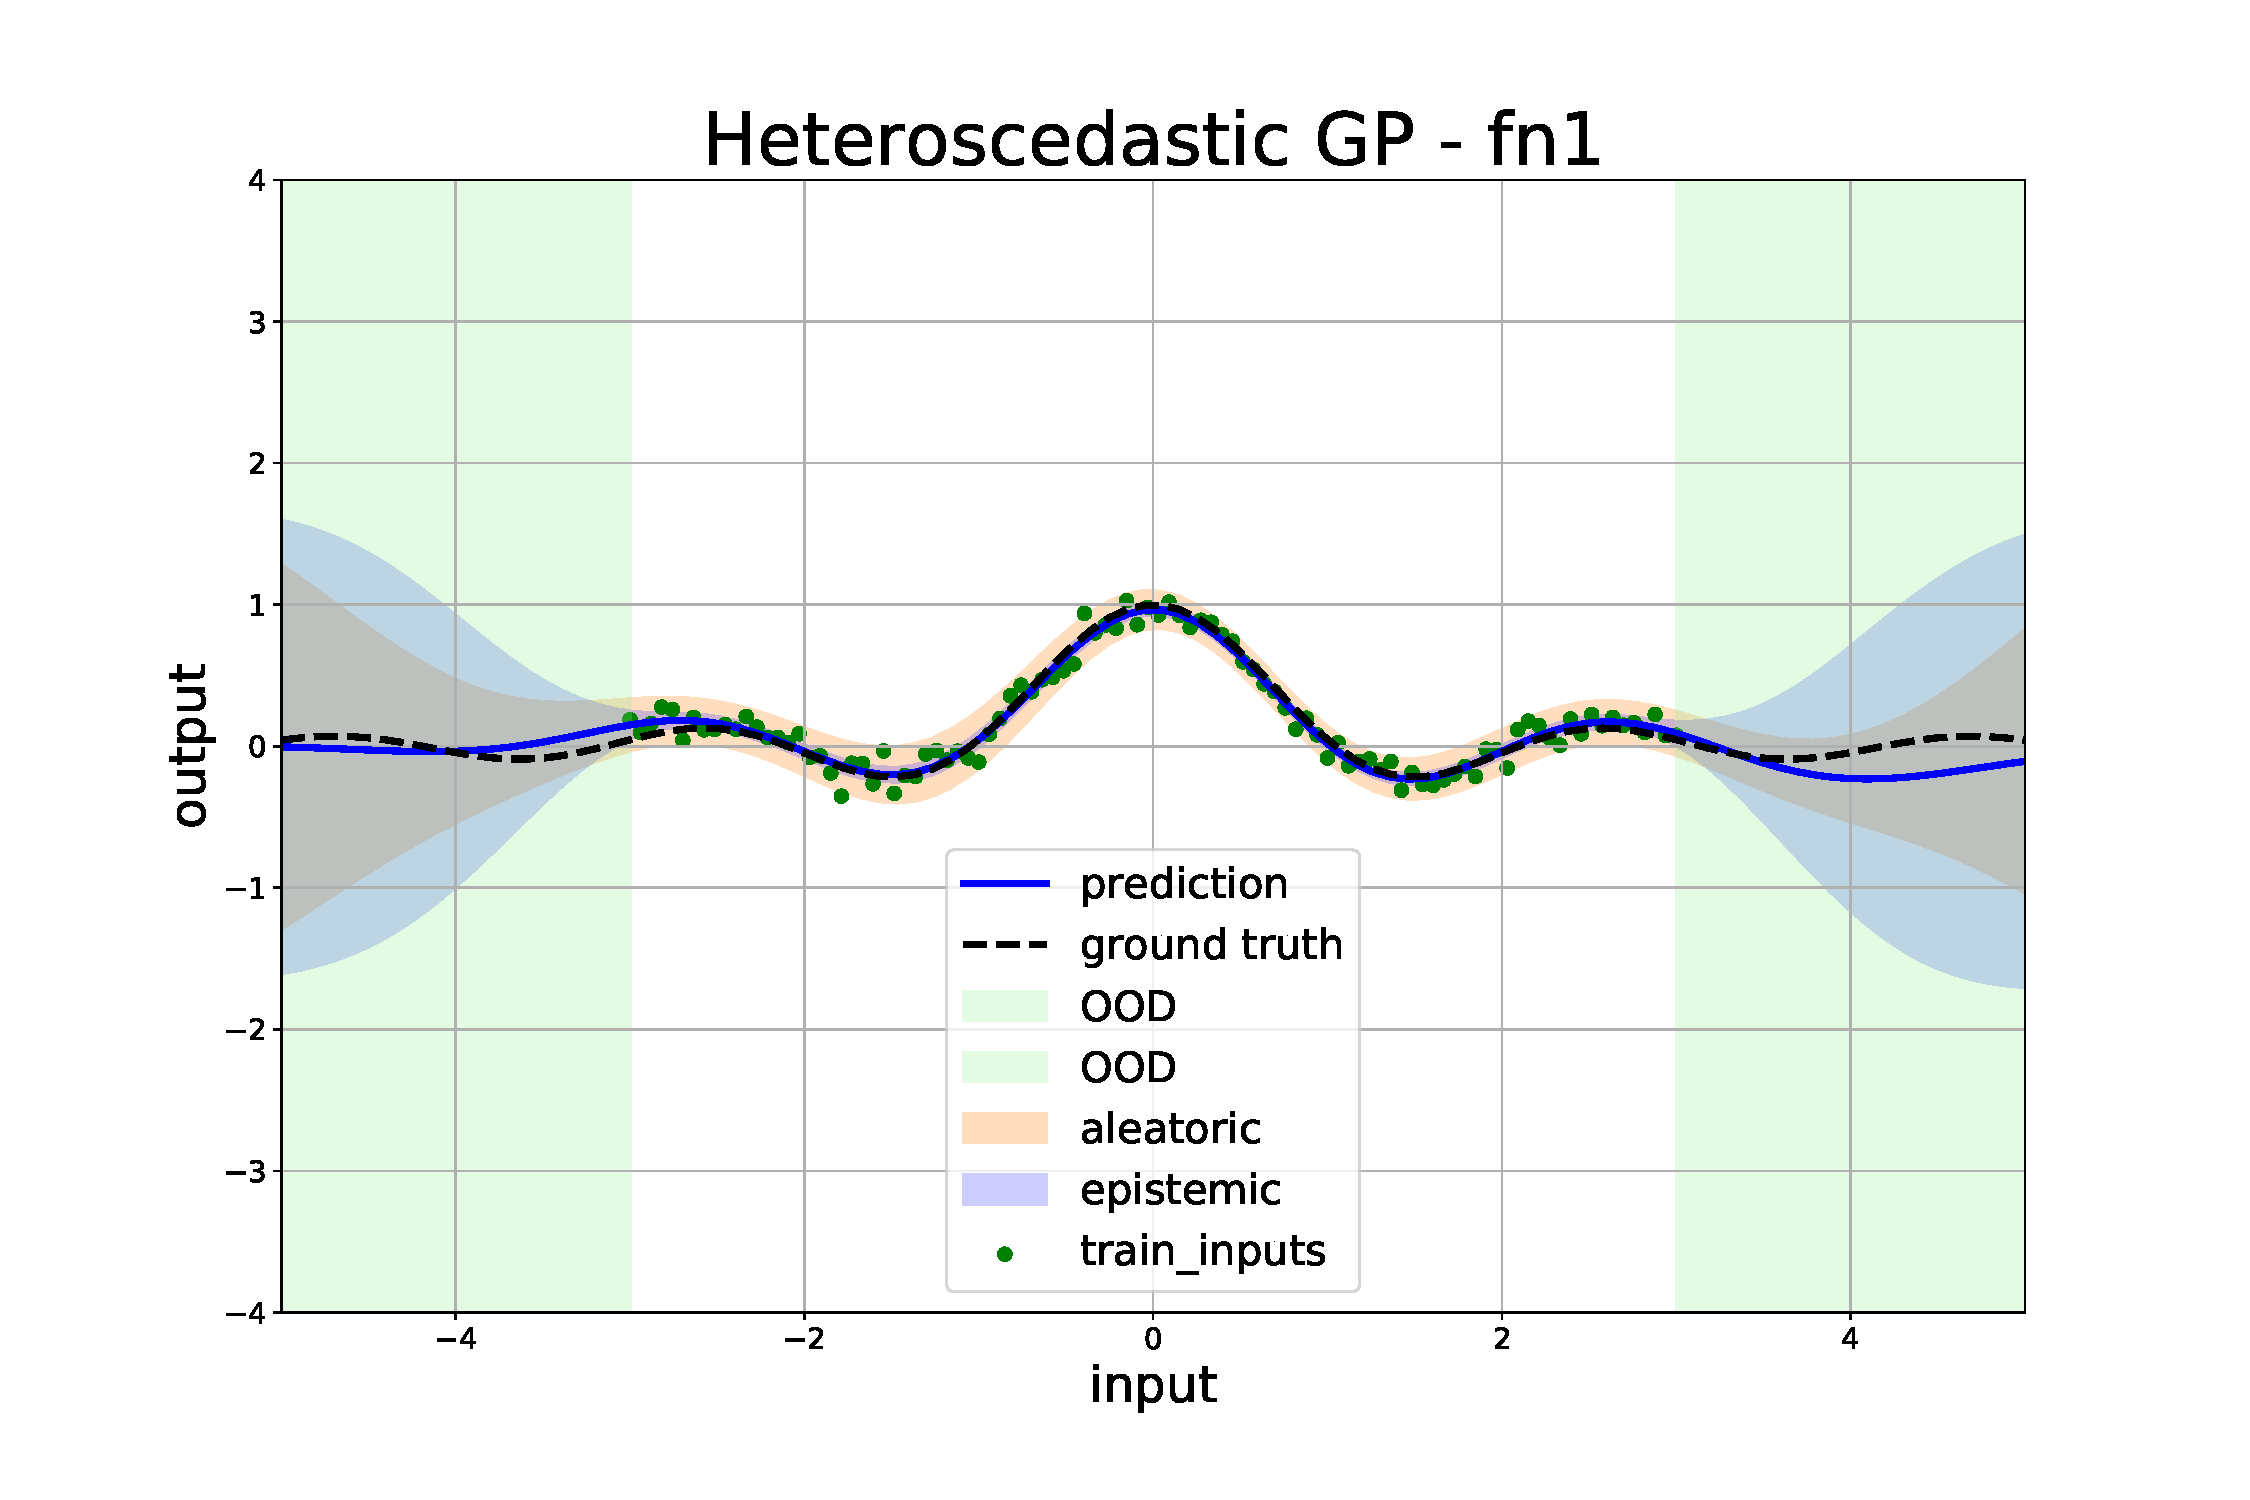
\includegraphics[width=\textwidth]{toy_dataset/hetero_fn1}
	\caption{$\epsilon=0.06$}
	\label{fig:five over x}
	\end{subfigure}
	\hfill
	\begin{subfigure}[b]{0.4\textwidth}
	\centering
	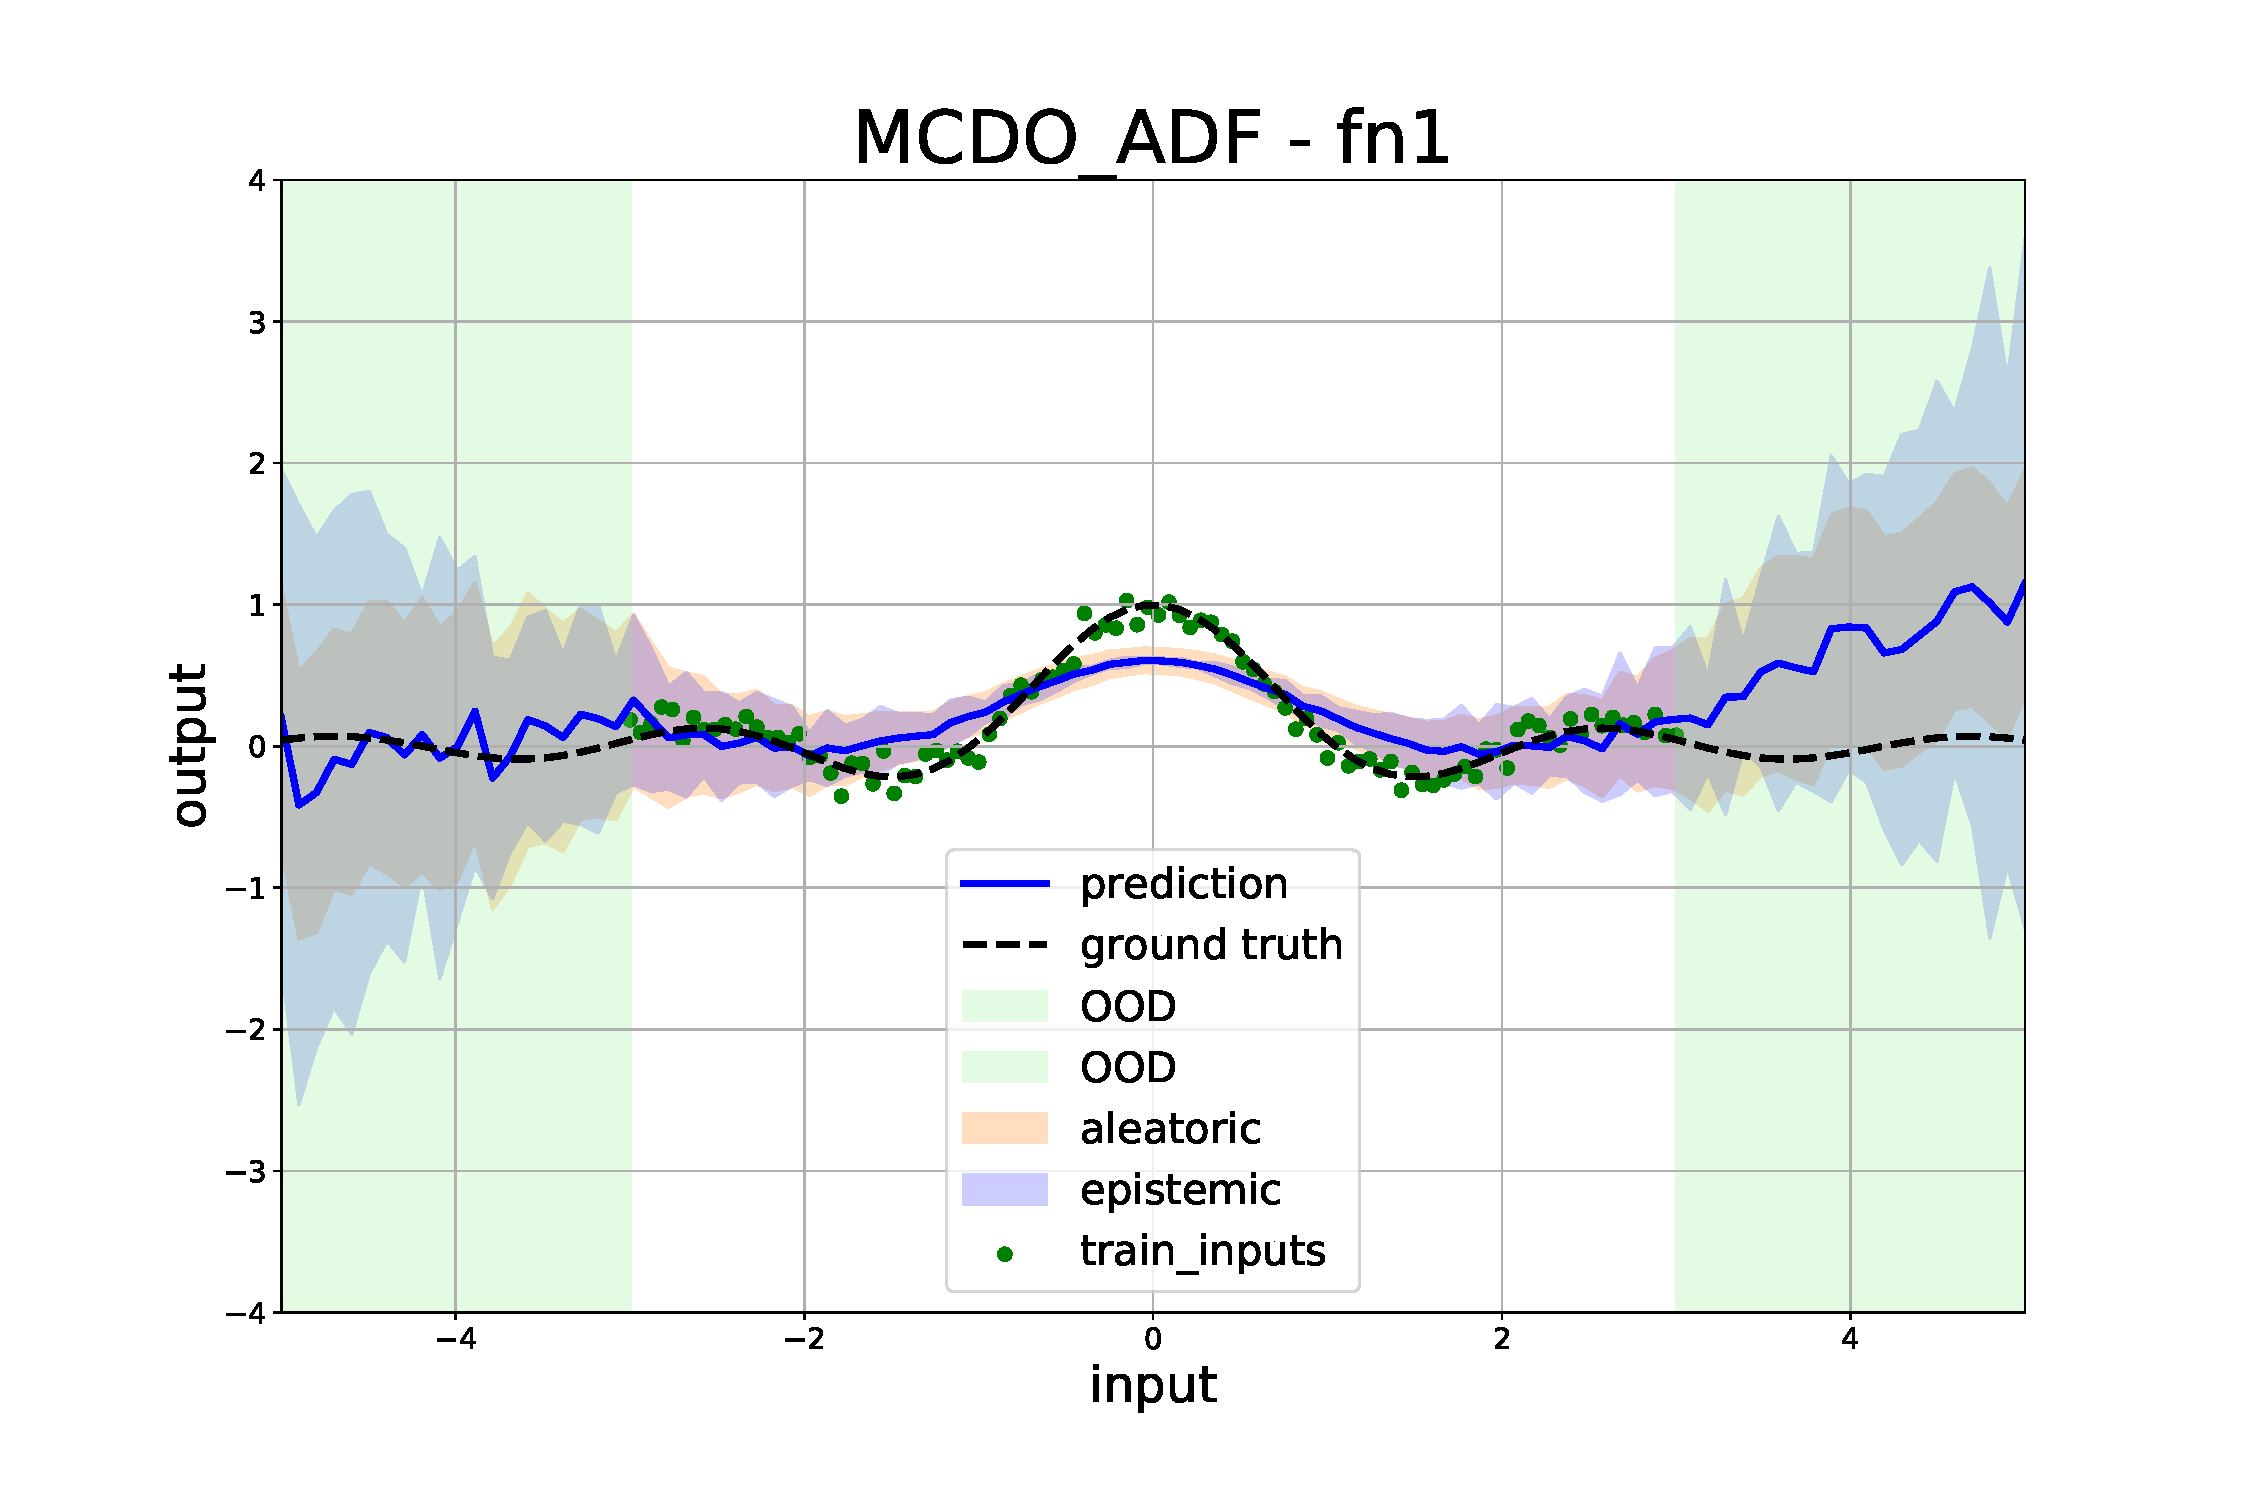
\includegraphics[width=\textwidth]{toy_dataset/mcdo_fn1}
	\caption{$\epsilon=0.02$}
	\label{fig:three sin x}
	\end{subfigure}
	\hfill
	\begin{subfigure}[b]{0.4\textwidth}
	\centering
	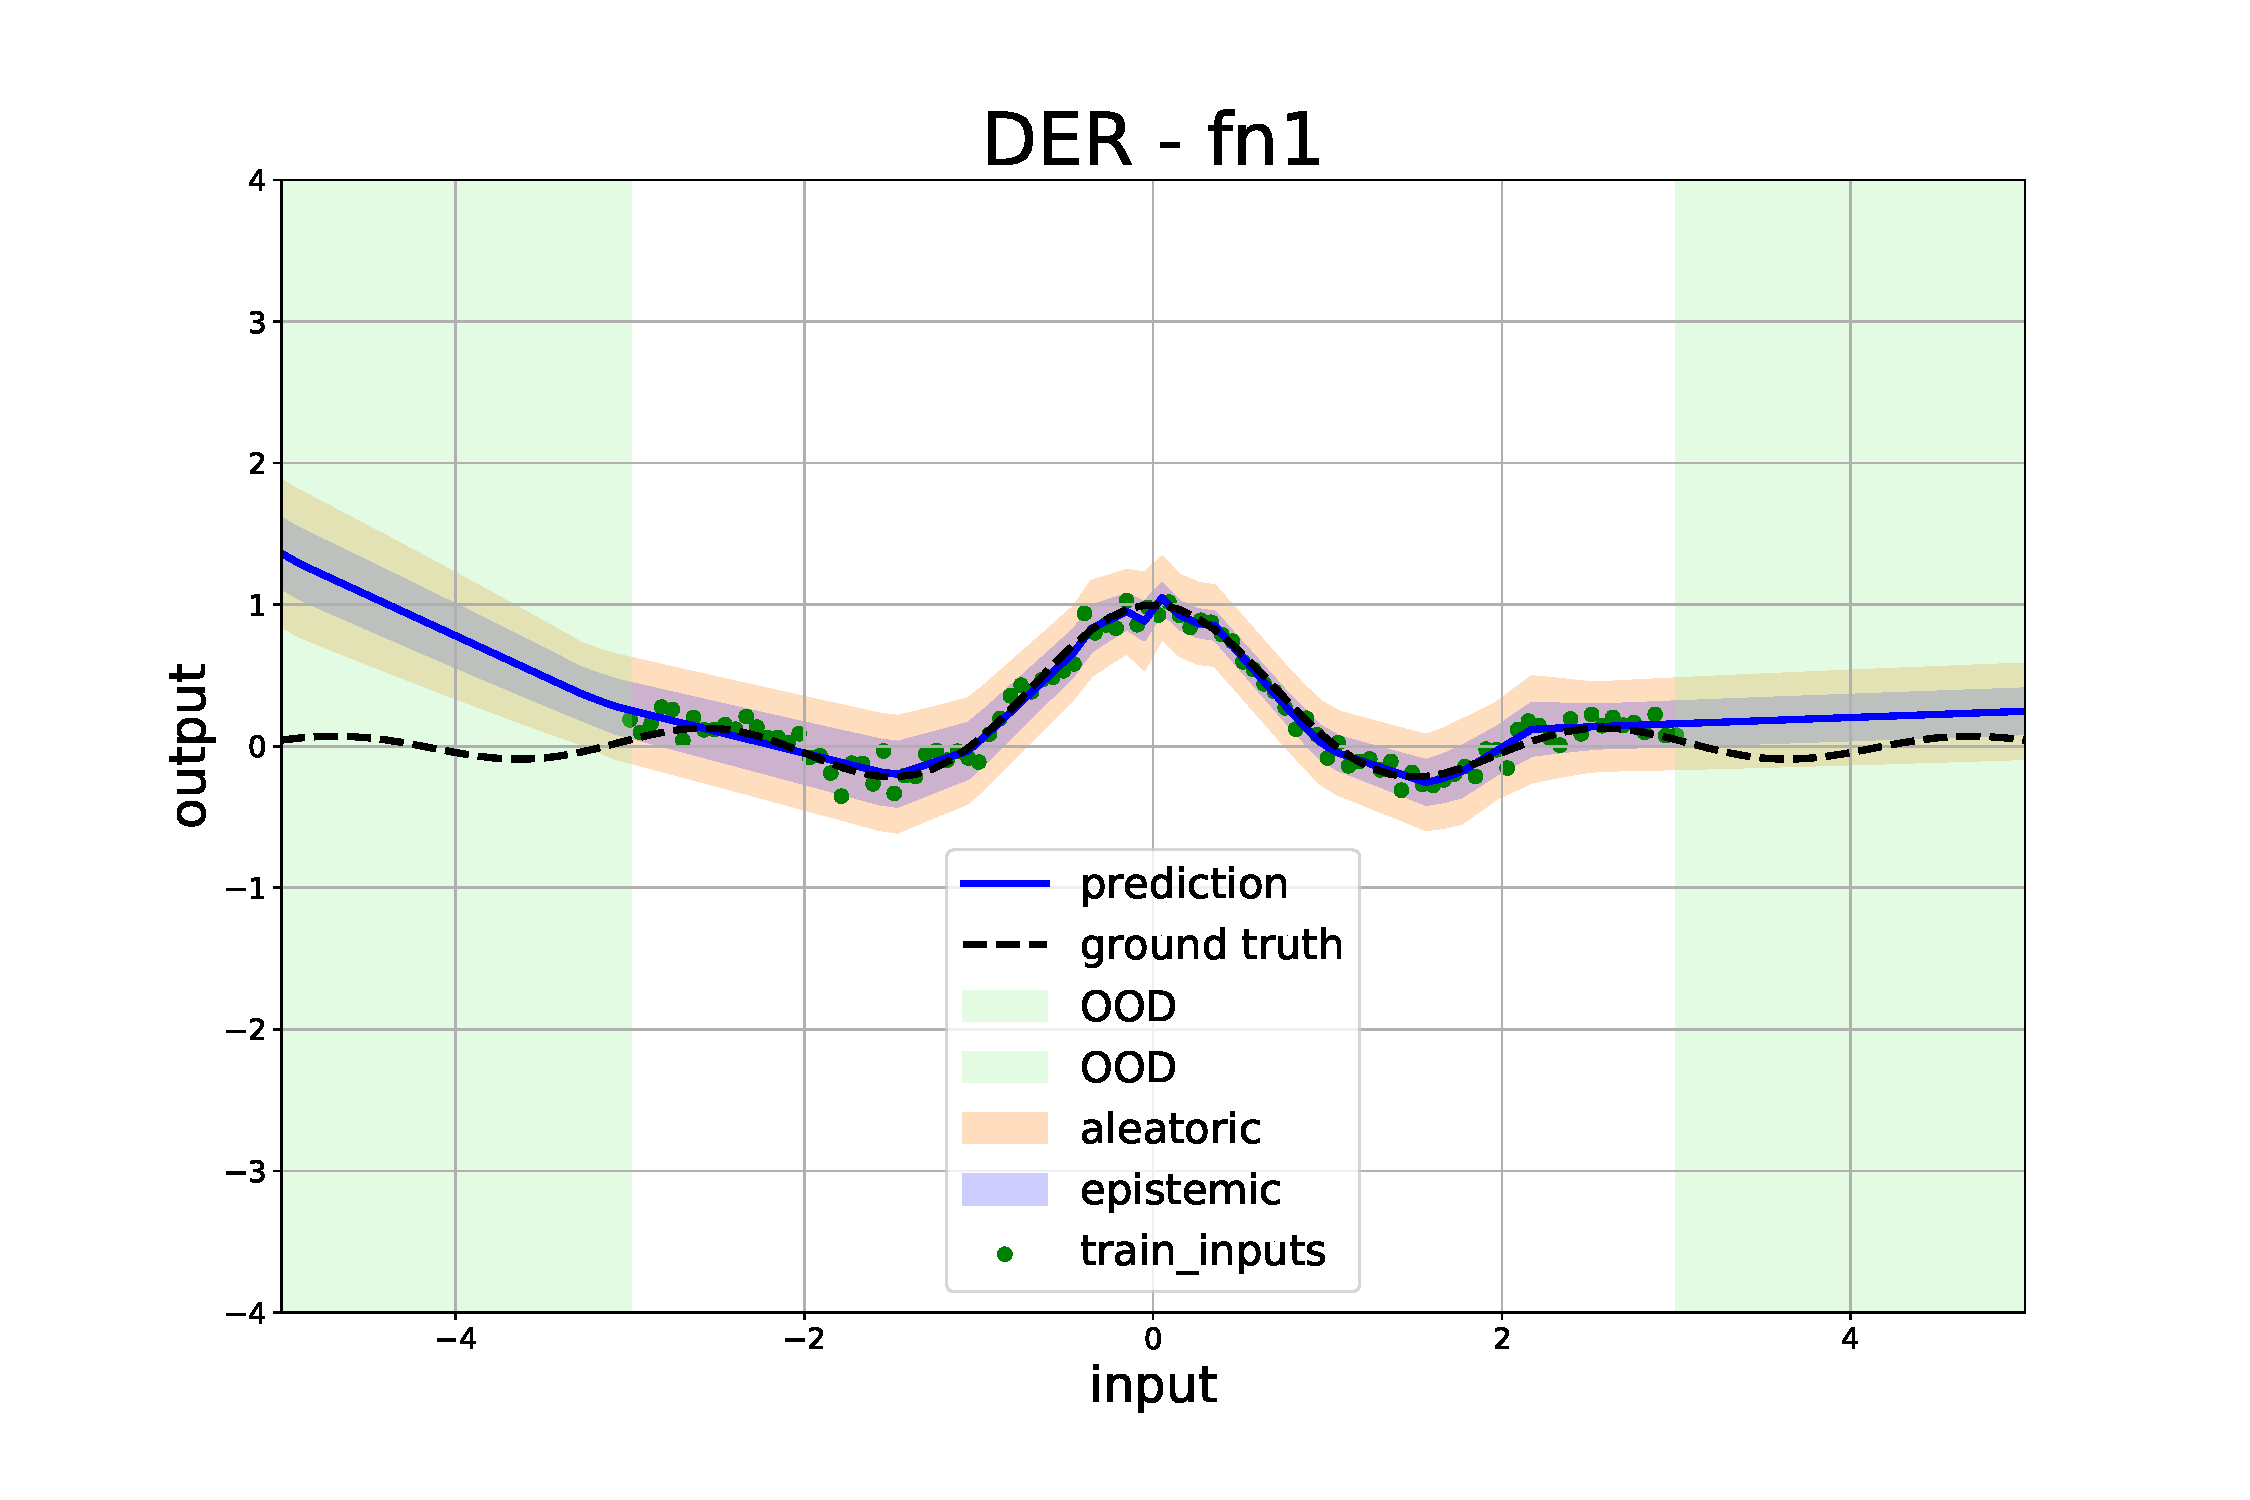
\includegraphics[width=\textwidth]{toy_dataset/der_fn1}
	\caption{$\epsilon=0.06$}
	\label{fig:five over x}
	\end{subfigure}
	\hfill
	\begin{subfigure}[b]{0.4\textwidth}
	\centering
	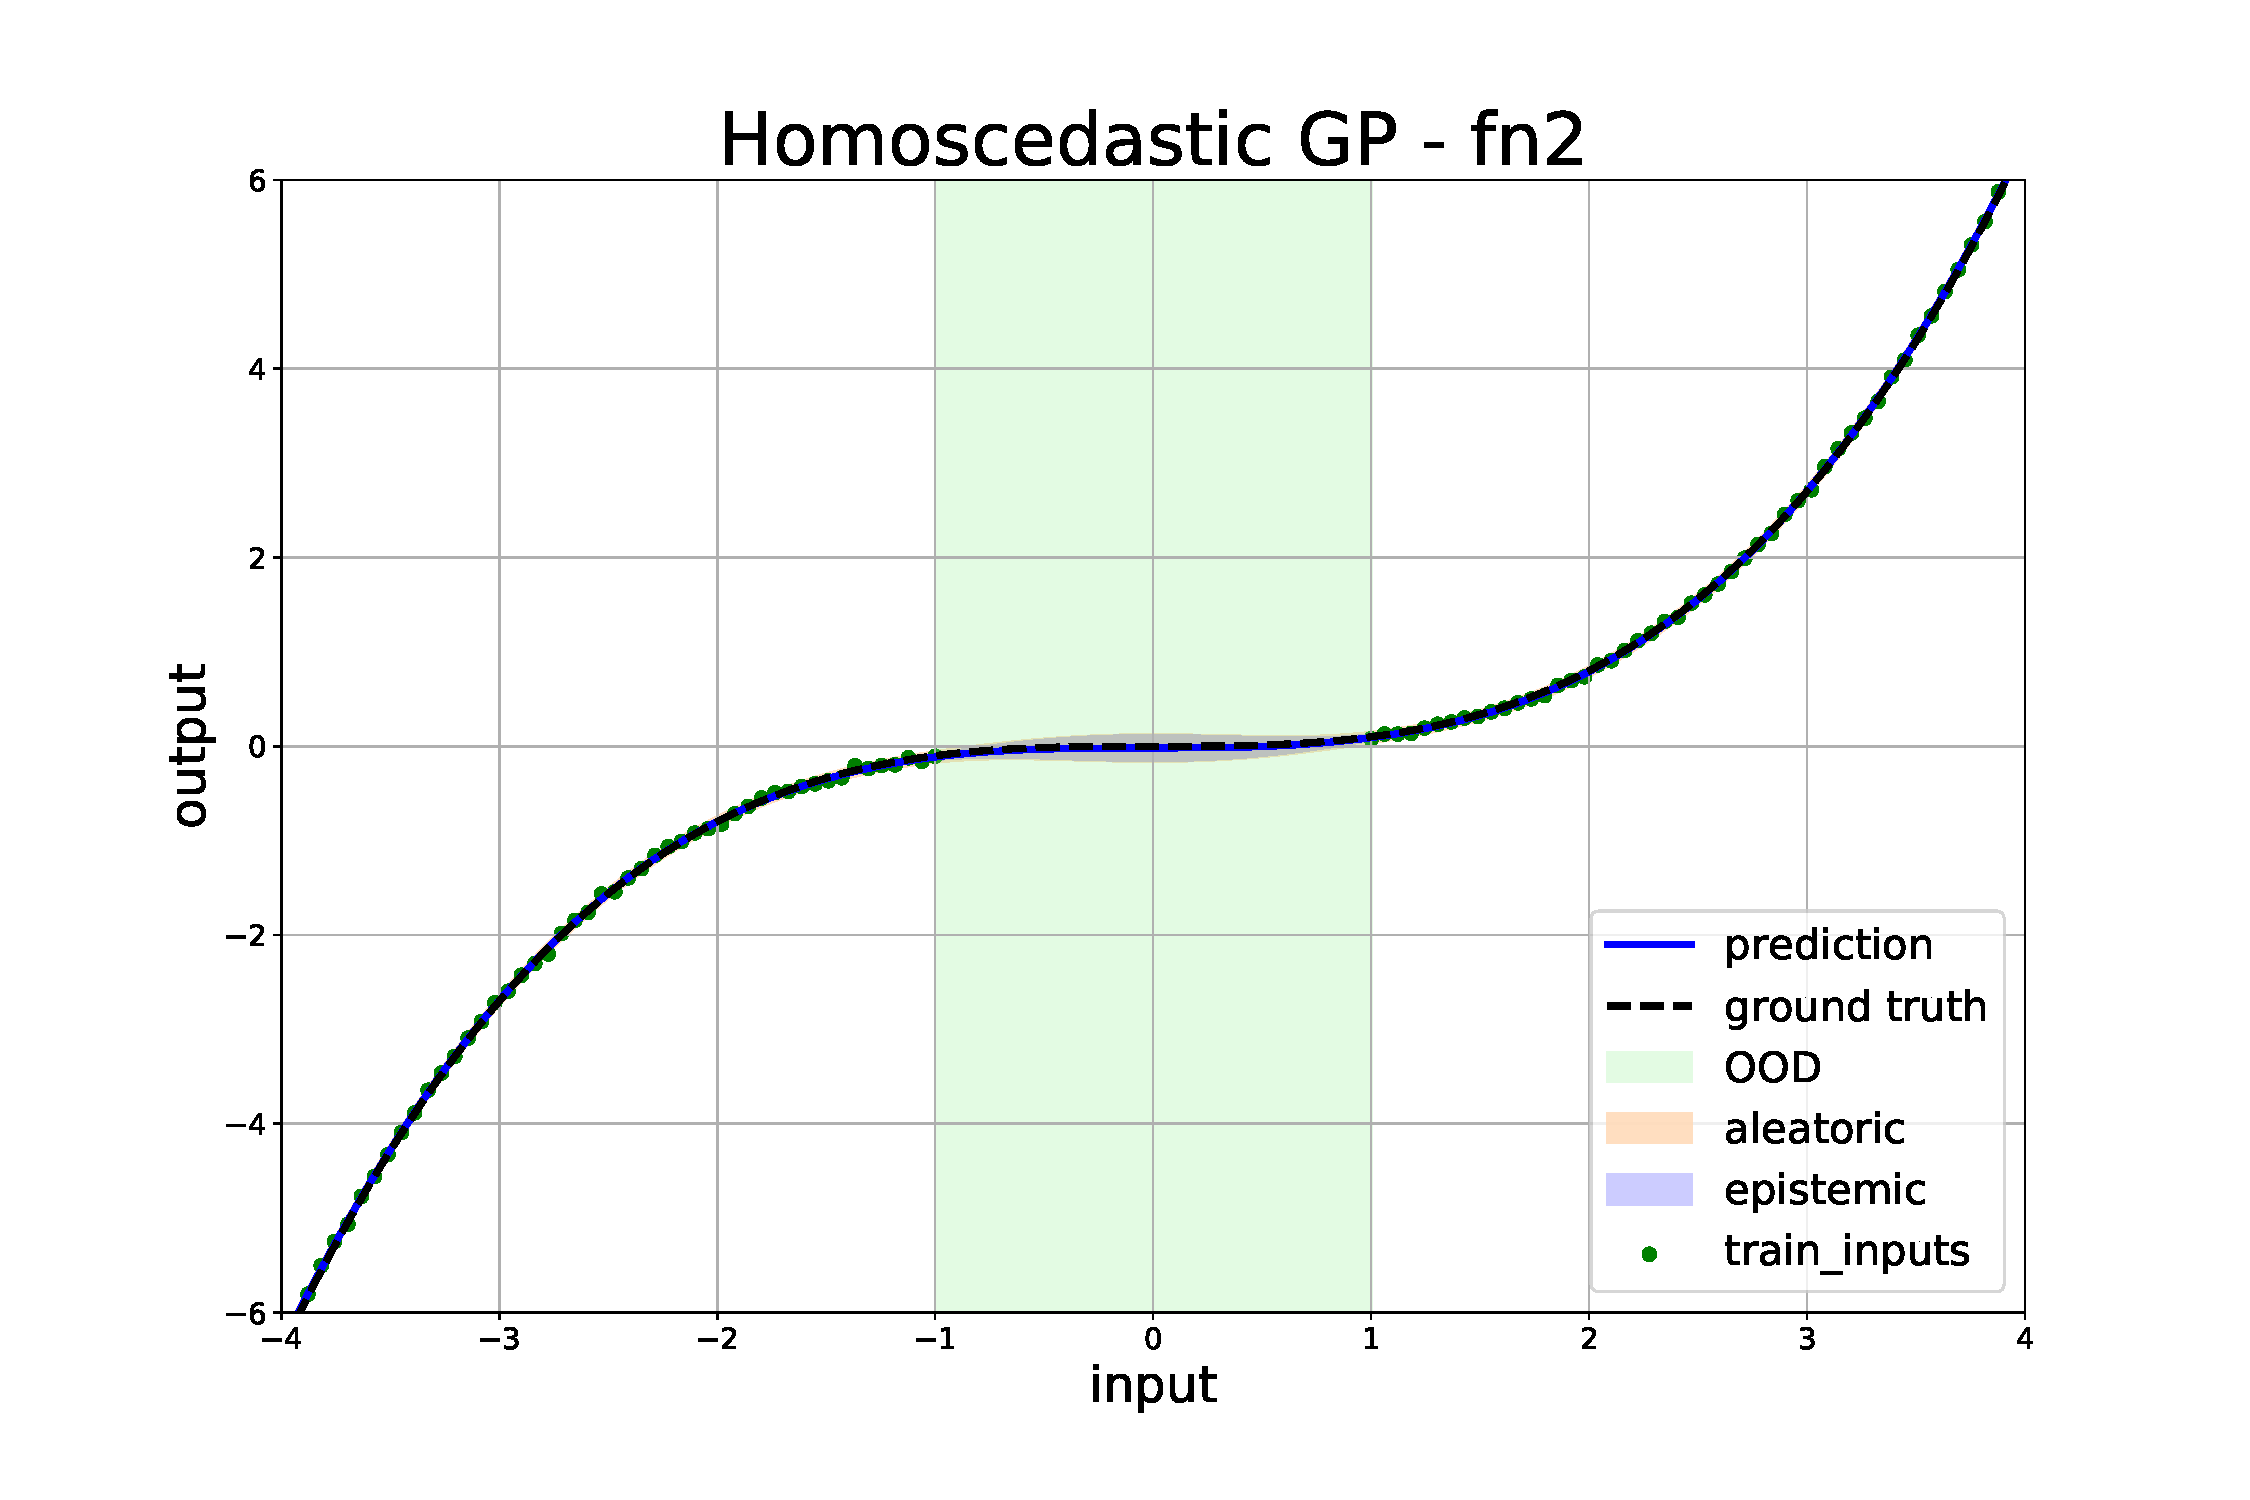
\includegraphics[width=\textwidth]{toy_dataset/homo_fn2}
	\caption{$\epsilon=0.06$}
	\label{fig:five over x}
	\end{subfigure}
	\hfill
	\begin{subfigure}[b]{0.4\textwidth}
	\centering
	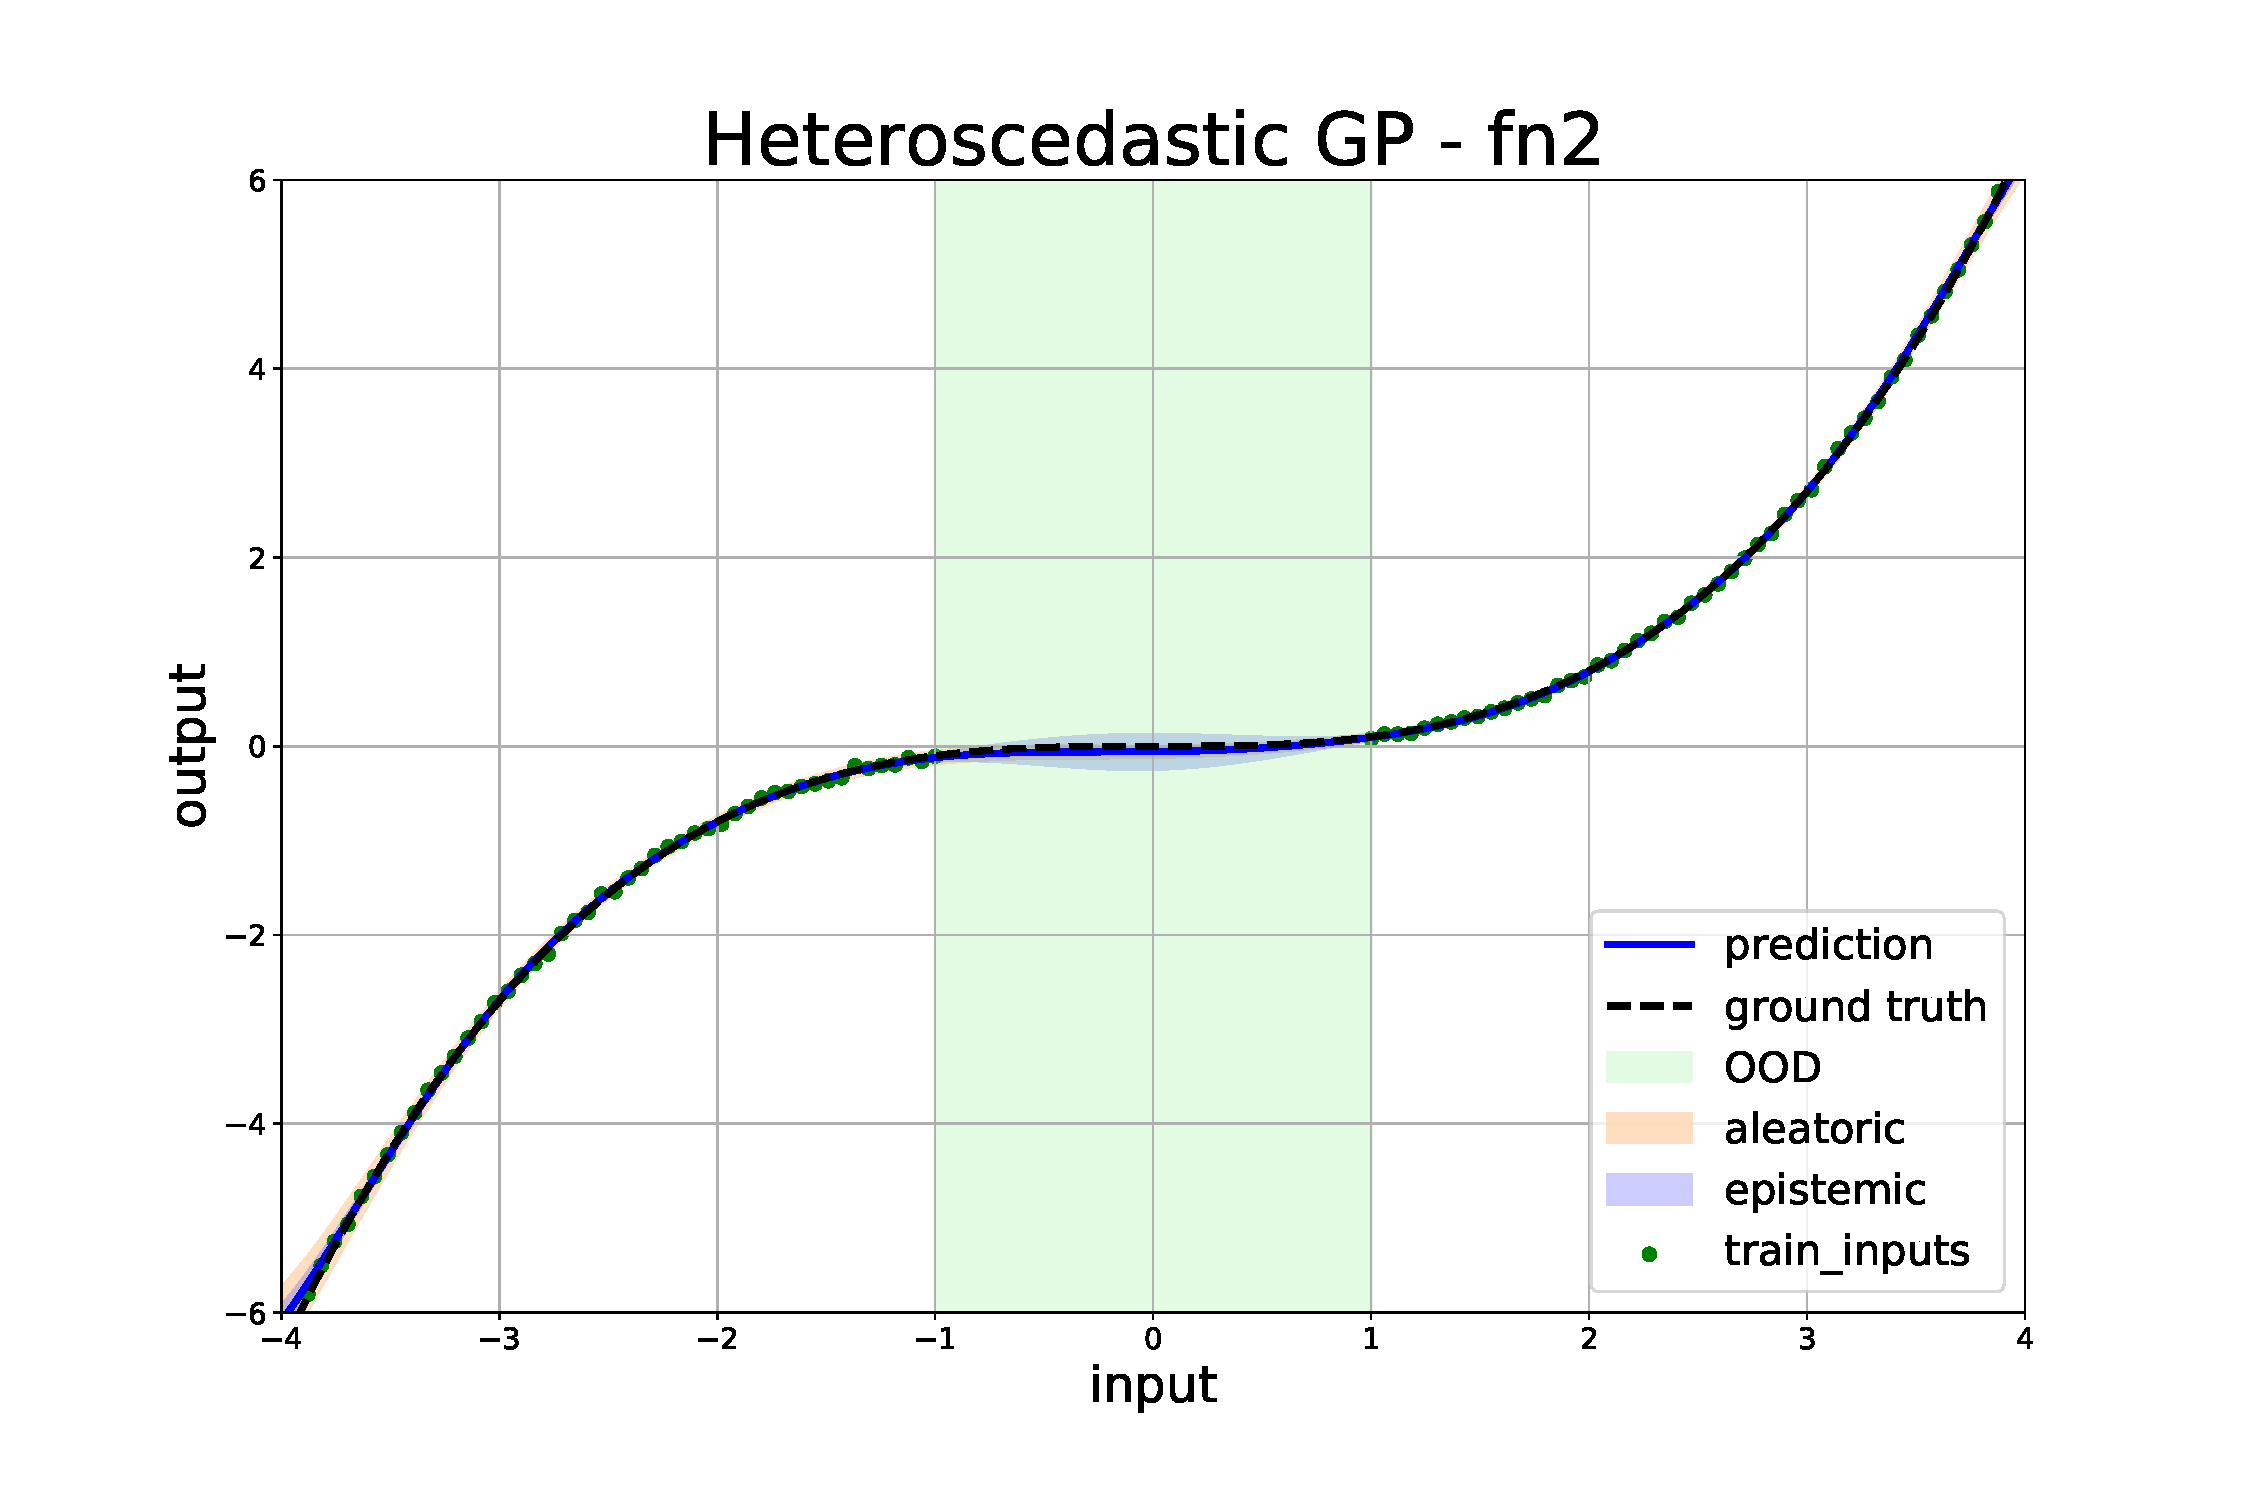
\includegraphics[width=\textwidth]{toy_dataset/hetero_fn2}
	\caption{$\epsilon=0.06$}
	\label{fig:five over x}
	\end{subfigure}
\end{figure}

\begin{figure}[h]\ContinuedFloat
	\centering
	\begin{subfigure}[b]{0.4\textwidth}
	\centering
	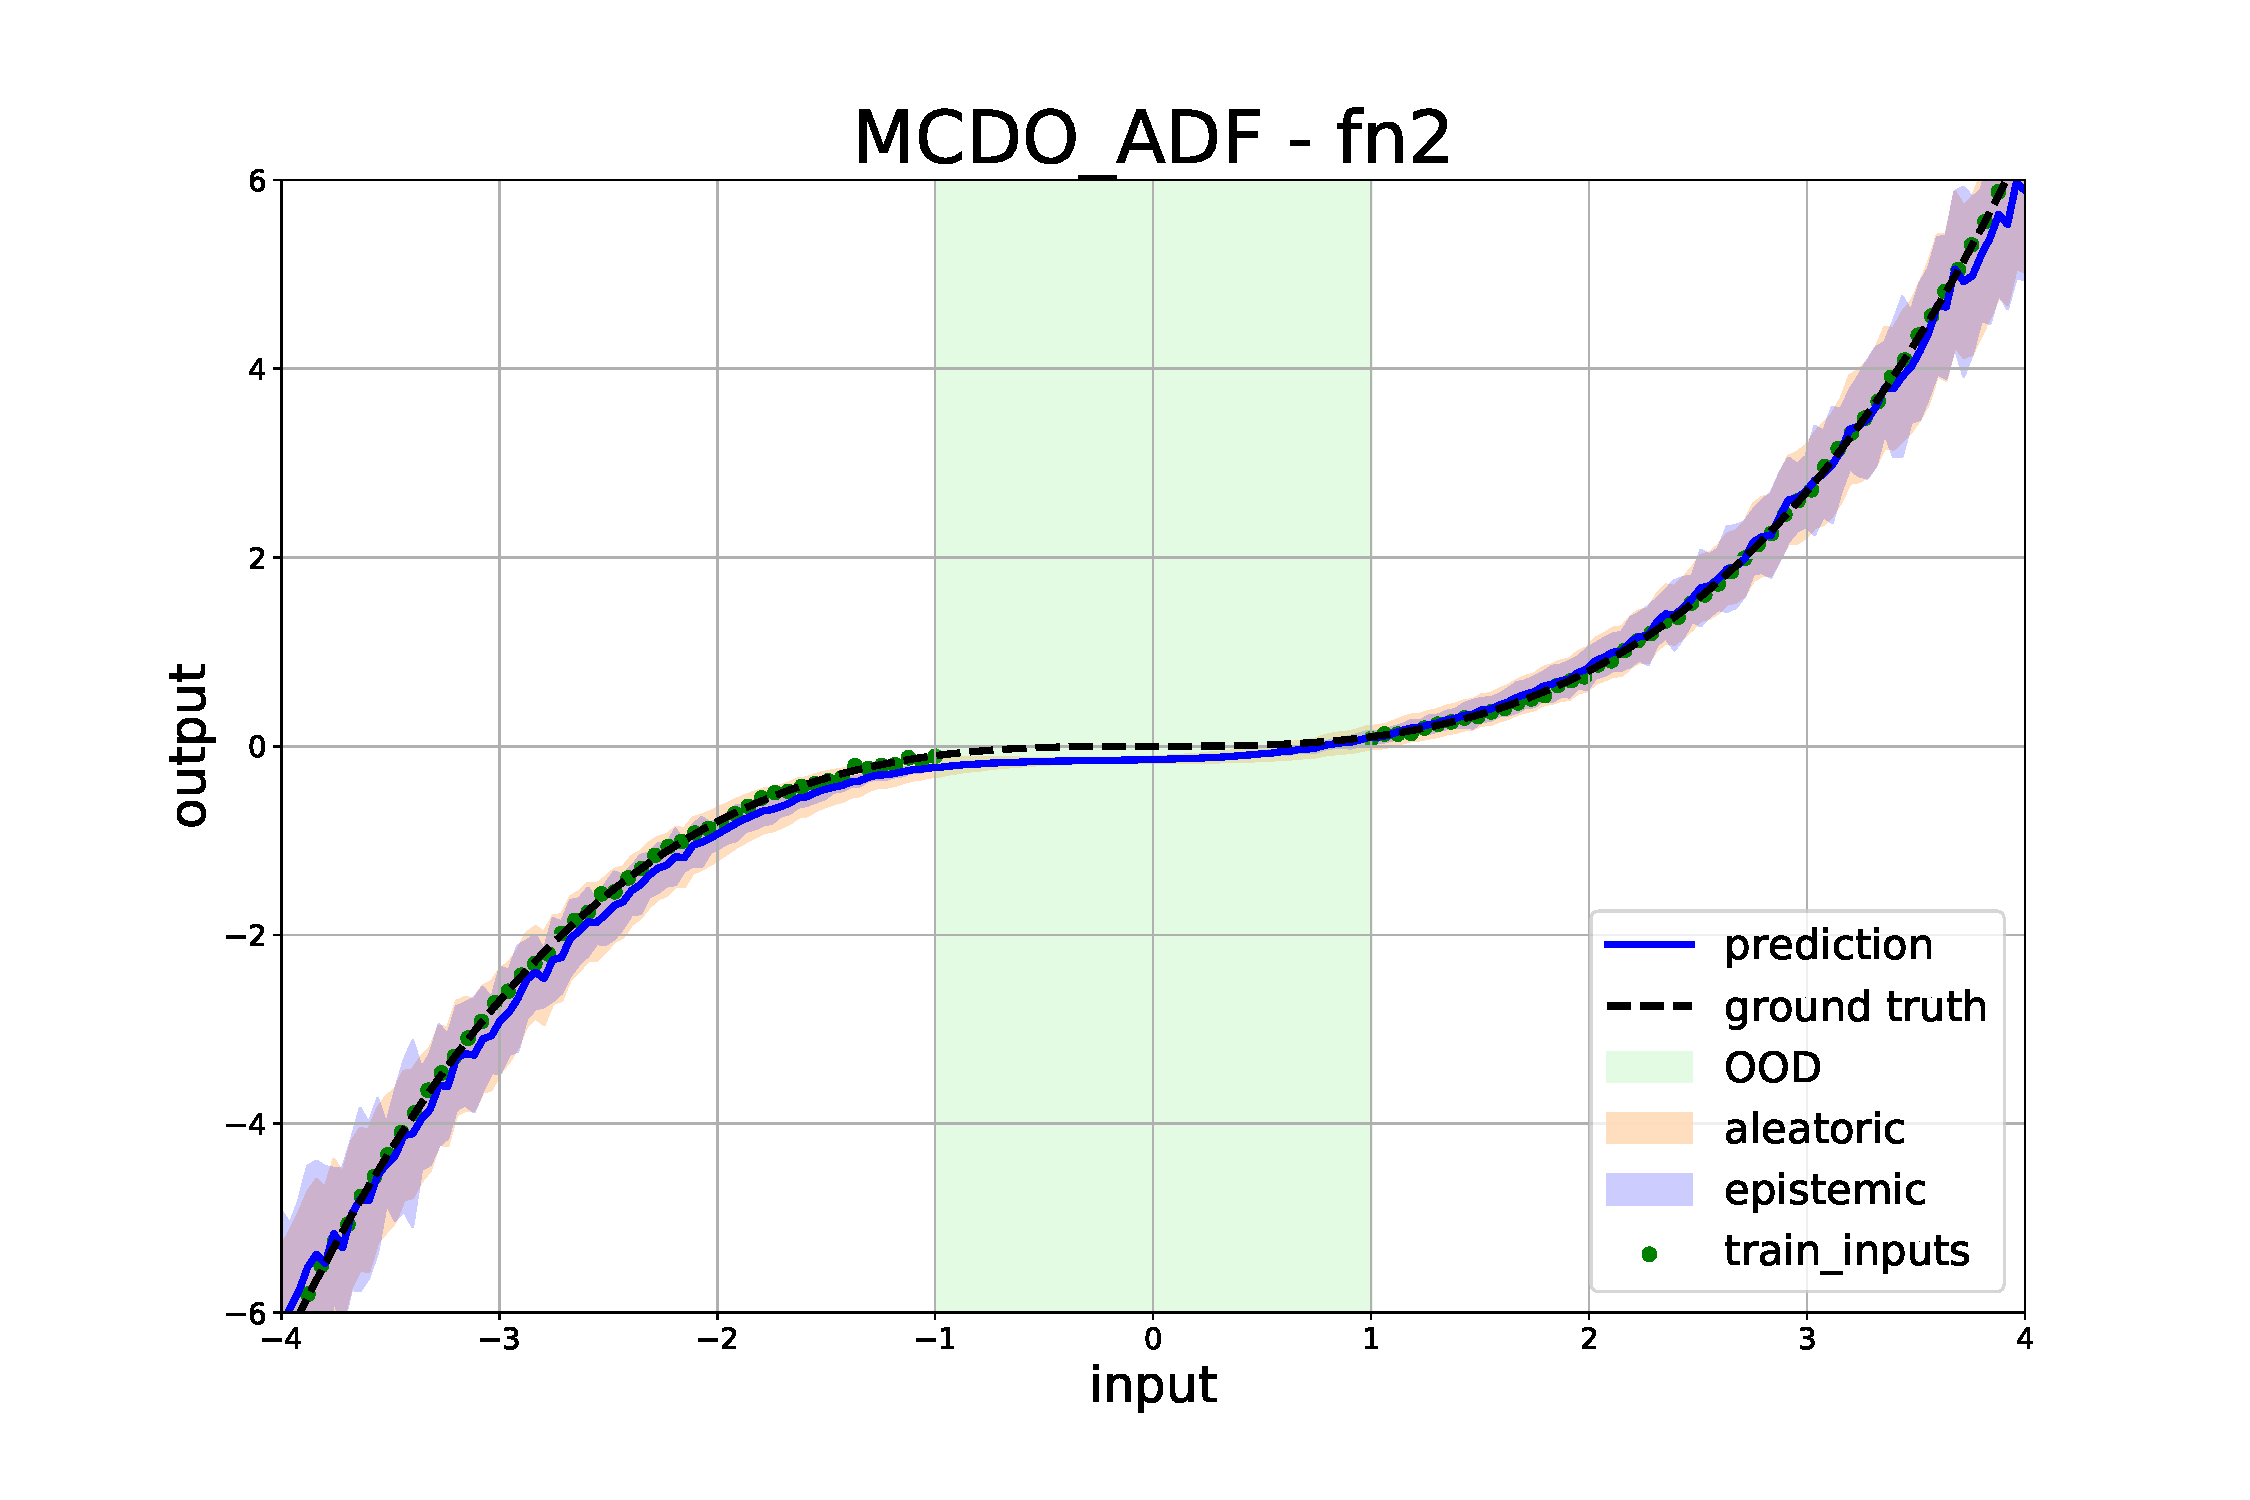
\includegraphics[width=\textwidth]{toy_dataset/mcdo_fn2}
	\caption{$\epsilon=0.06$}
	\label{fig:five over x}
	\end{subfigure}
	\hfill
	\begin{subfigure}[b]{0.4\textwidth}
	\centering
	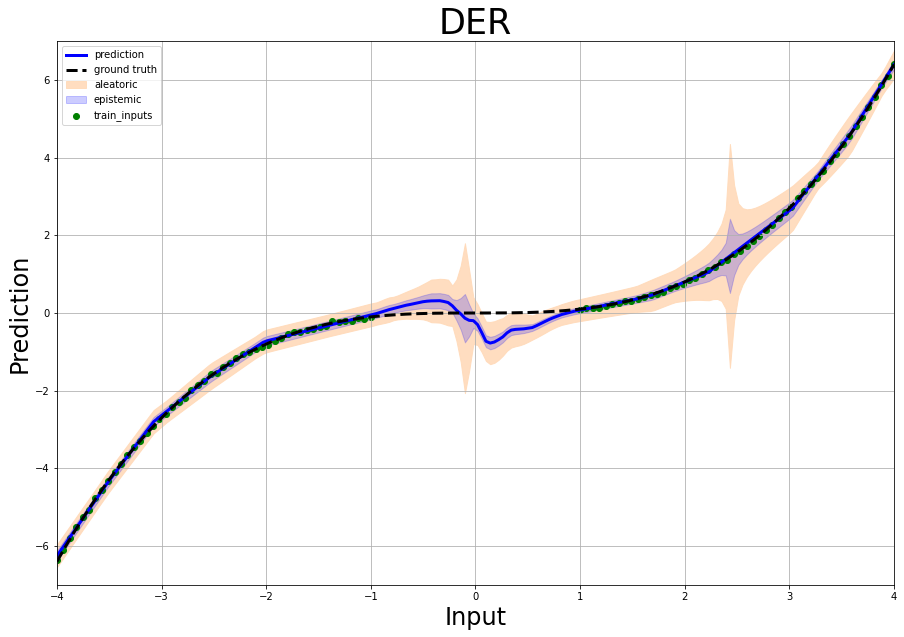
\includegraphics[width=\textwidth]{toy_dataset/der_fn2}
	\caption{$\epsilon=0.06$}
	\label{fig:five over x}
	\end{subfigure}
	\hfill
	\begin{subfigure}[b]{0.4\textwidth}
	\centering
	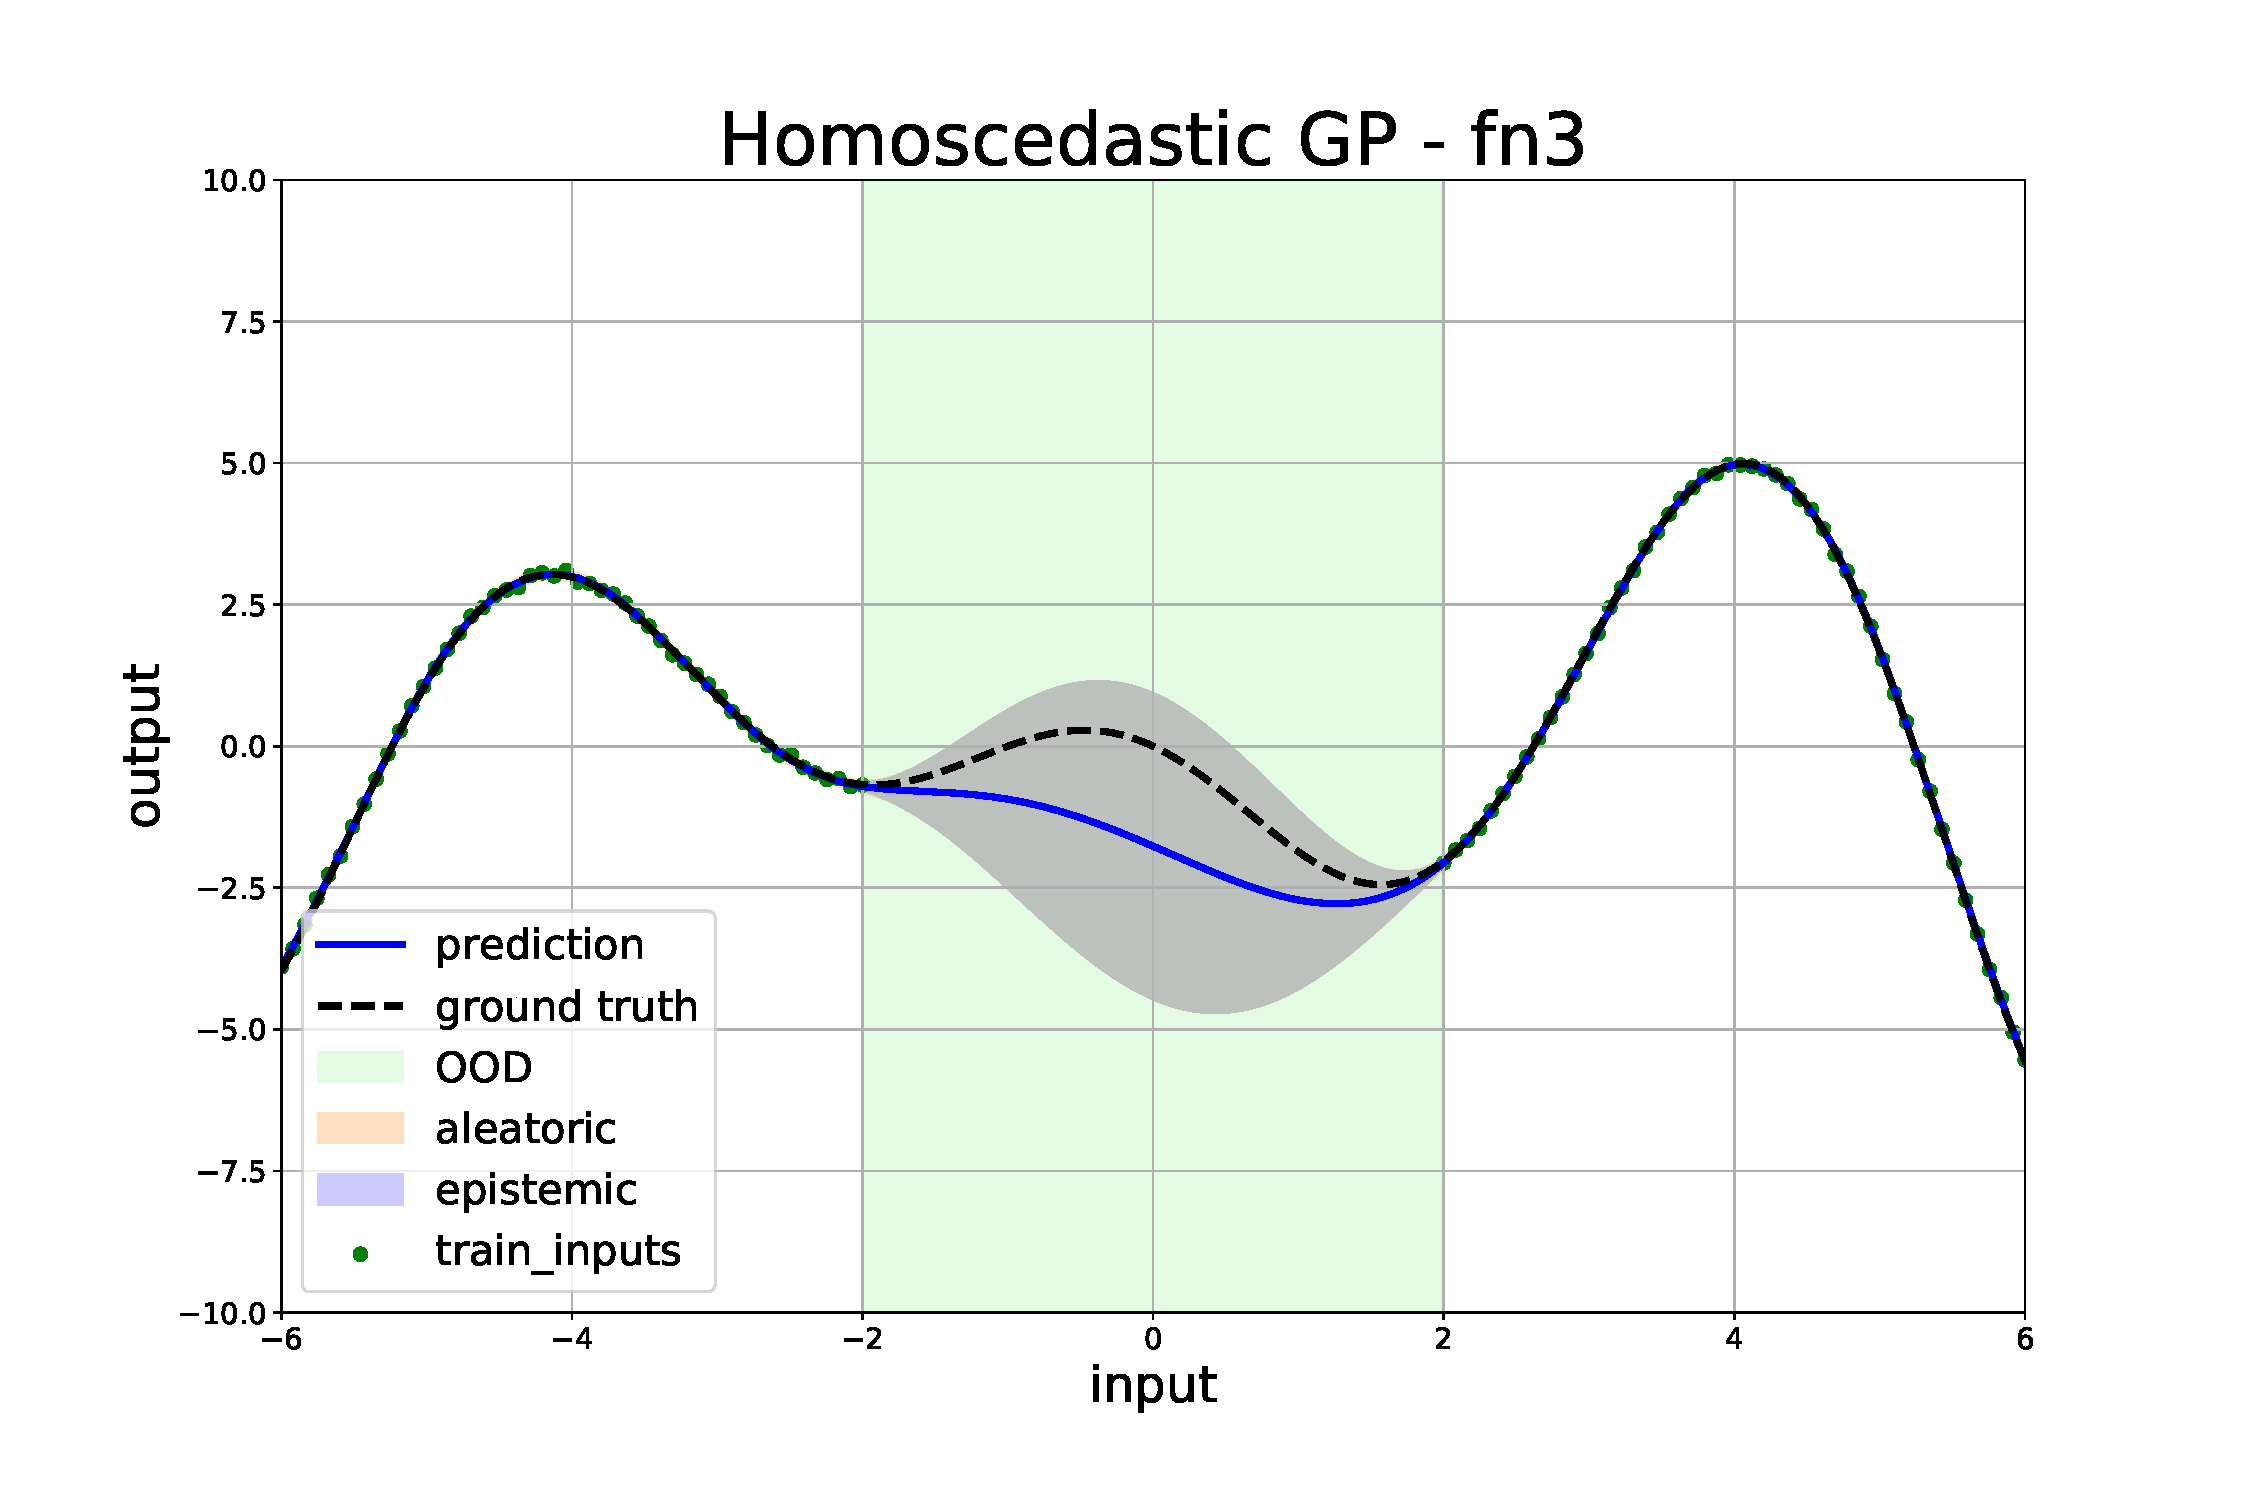
\includegraphics[width=\textwidth]{toy_dataset/homo_fn3}
	\caption{$\epsilon=0.06$}
	\label{fig:five over x}
	\end{subfigure}
	\hfill
	\begin{subfigure}[b]{0.4\textwidth}
	\centering
	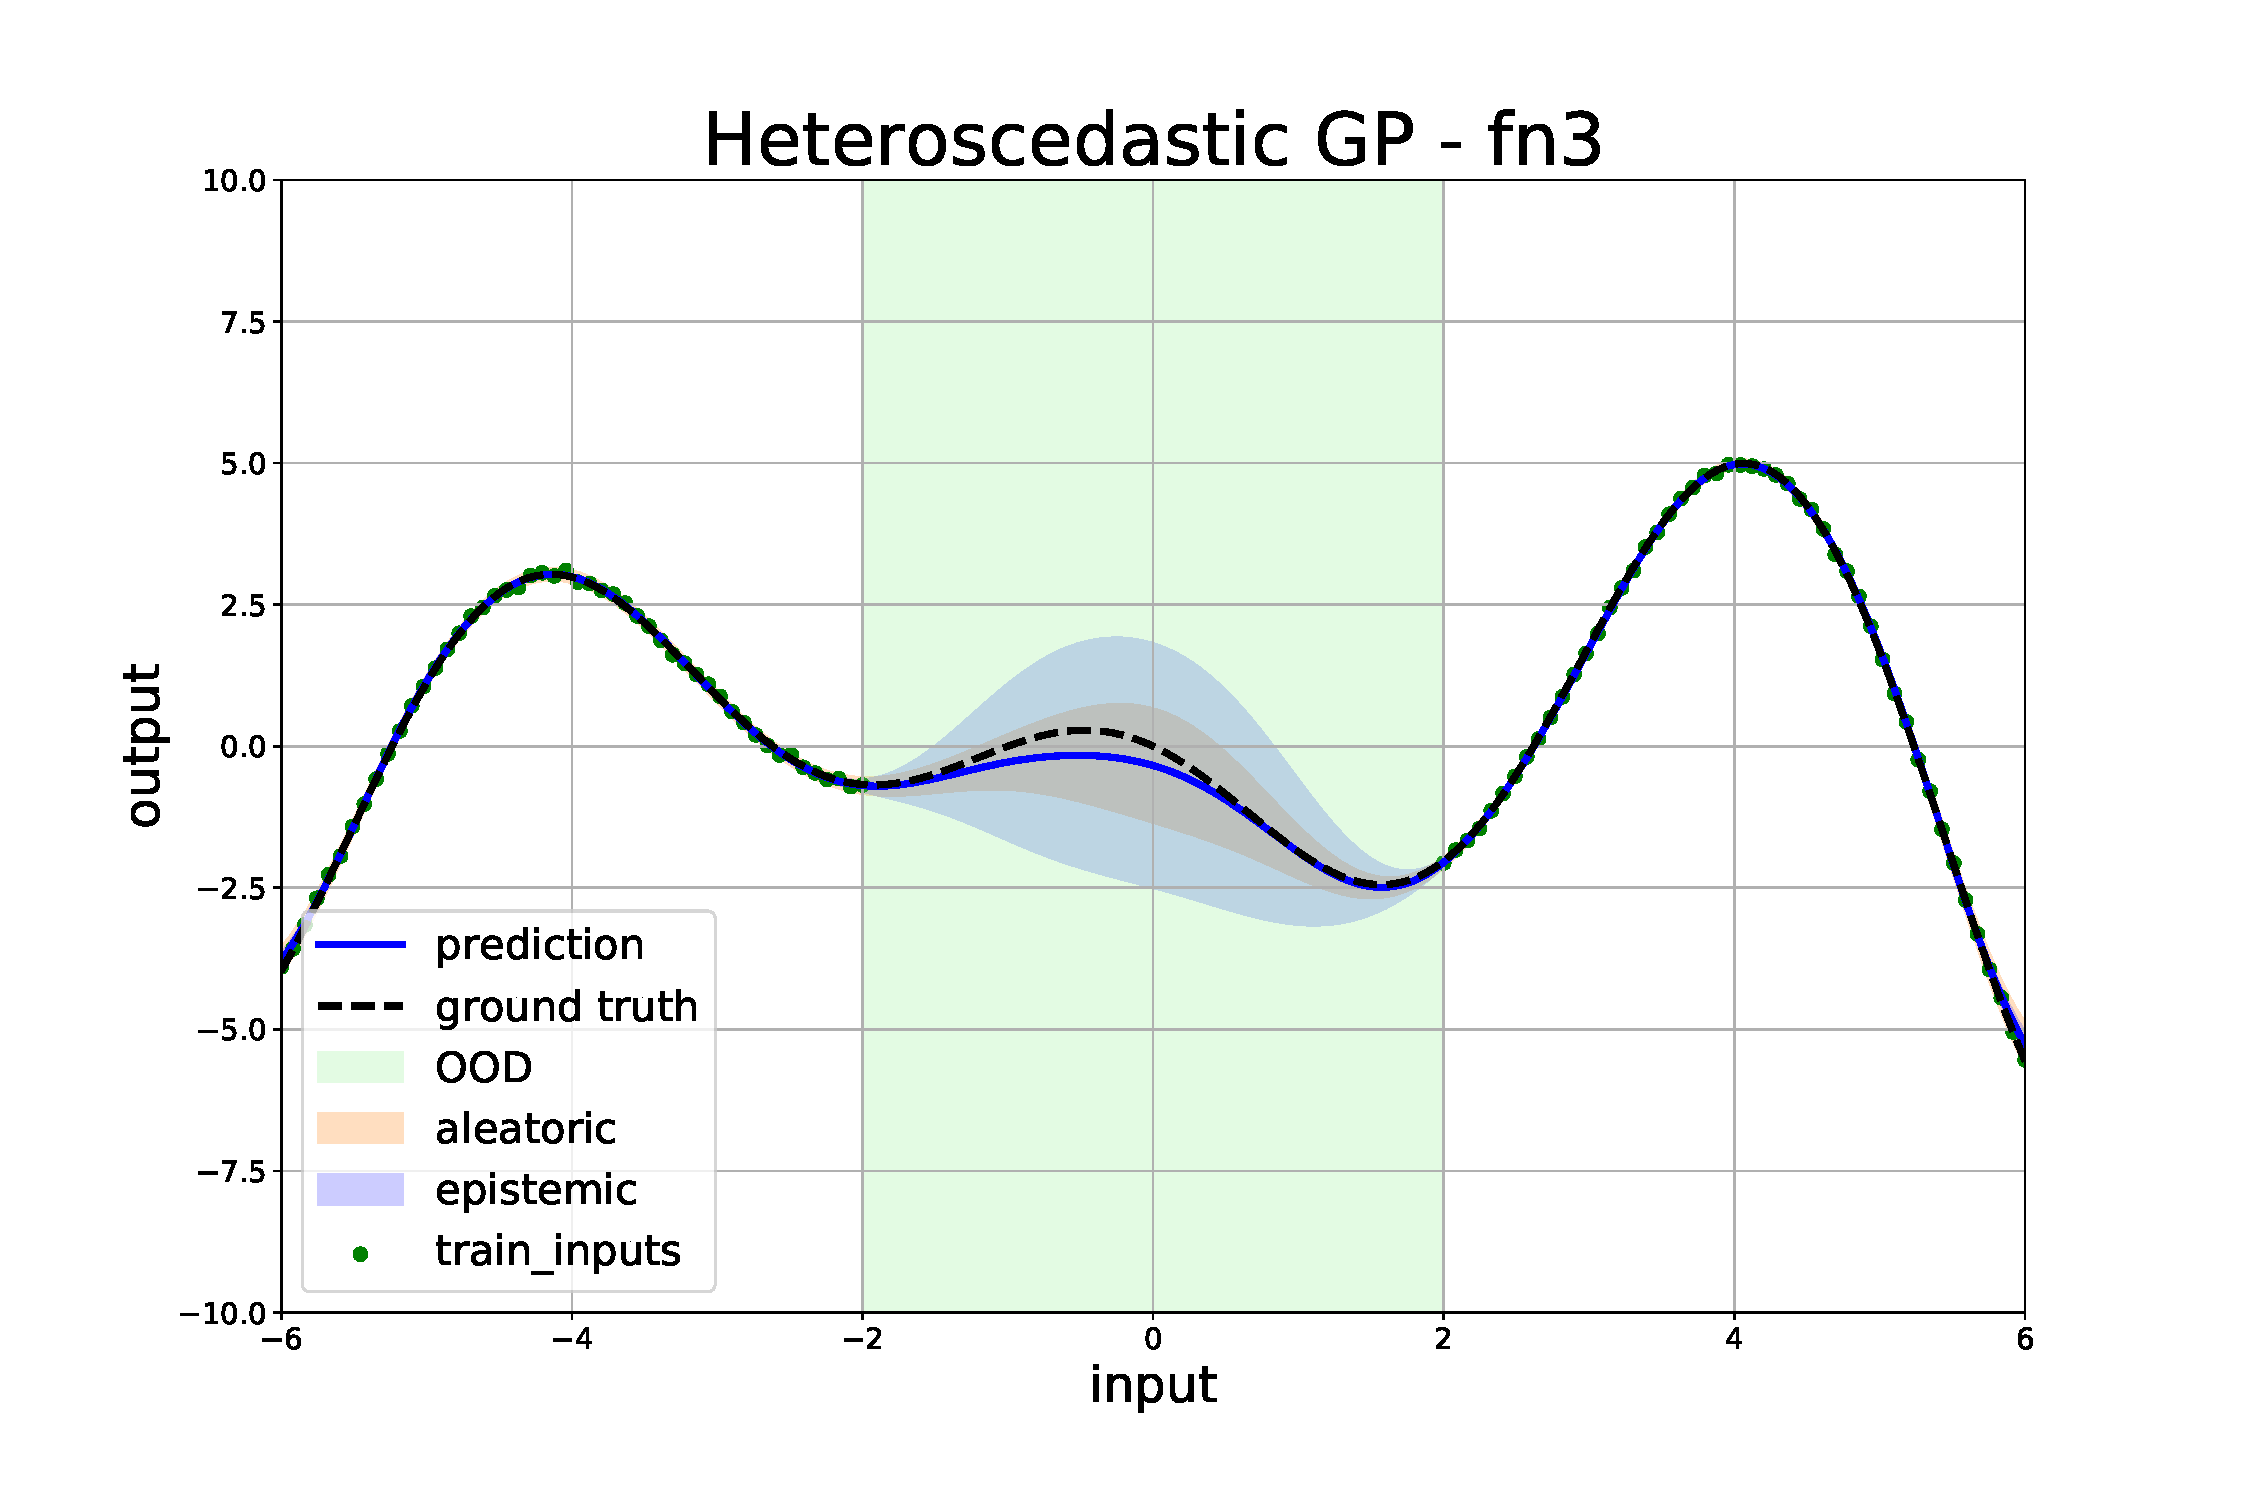
\includegraphics[width=\textwidth]{toy_dataset/hetero_fn3}
	\caption{$\epsilon=0.06$}
	\label{fig:five over x}
	\end{subfigure}
	\hfill
	\begin{subfigure}[b]{0.4\textwidth}
	\centering
	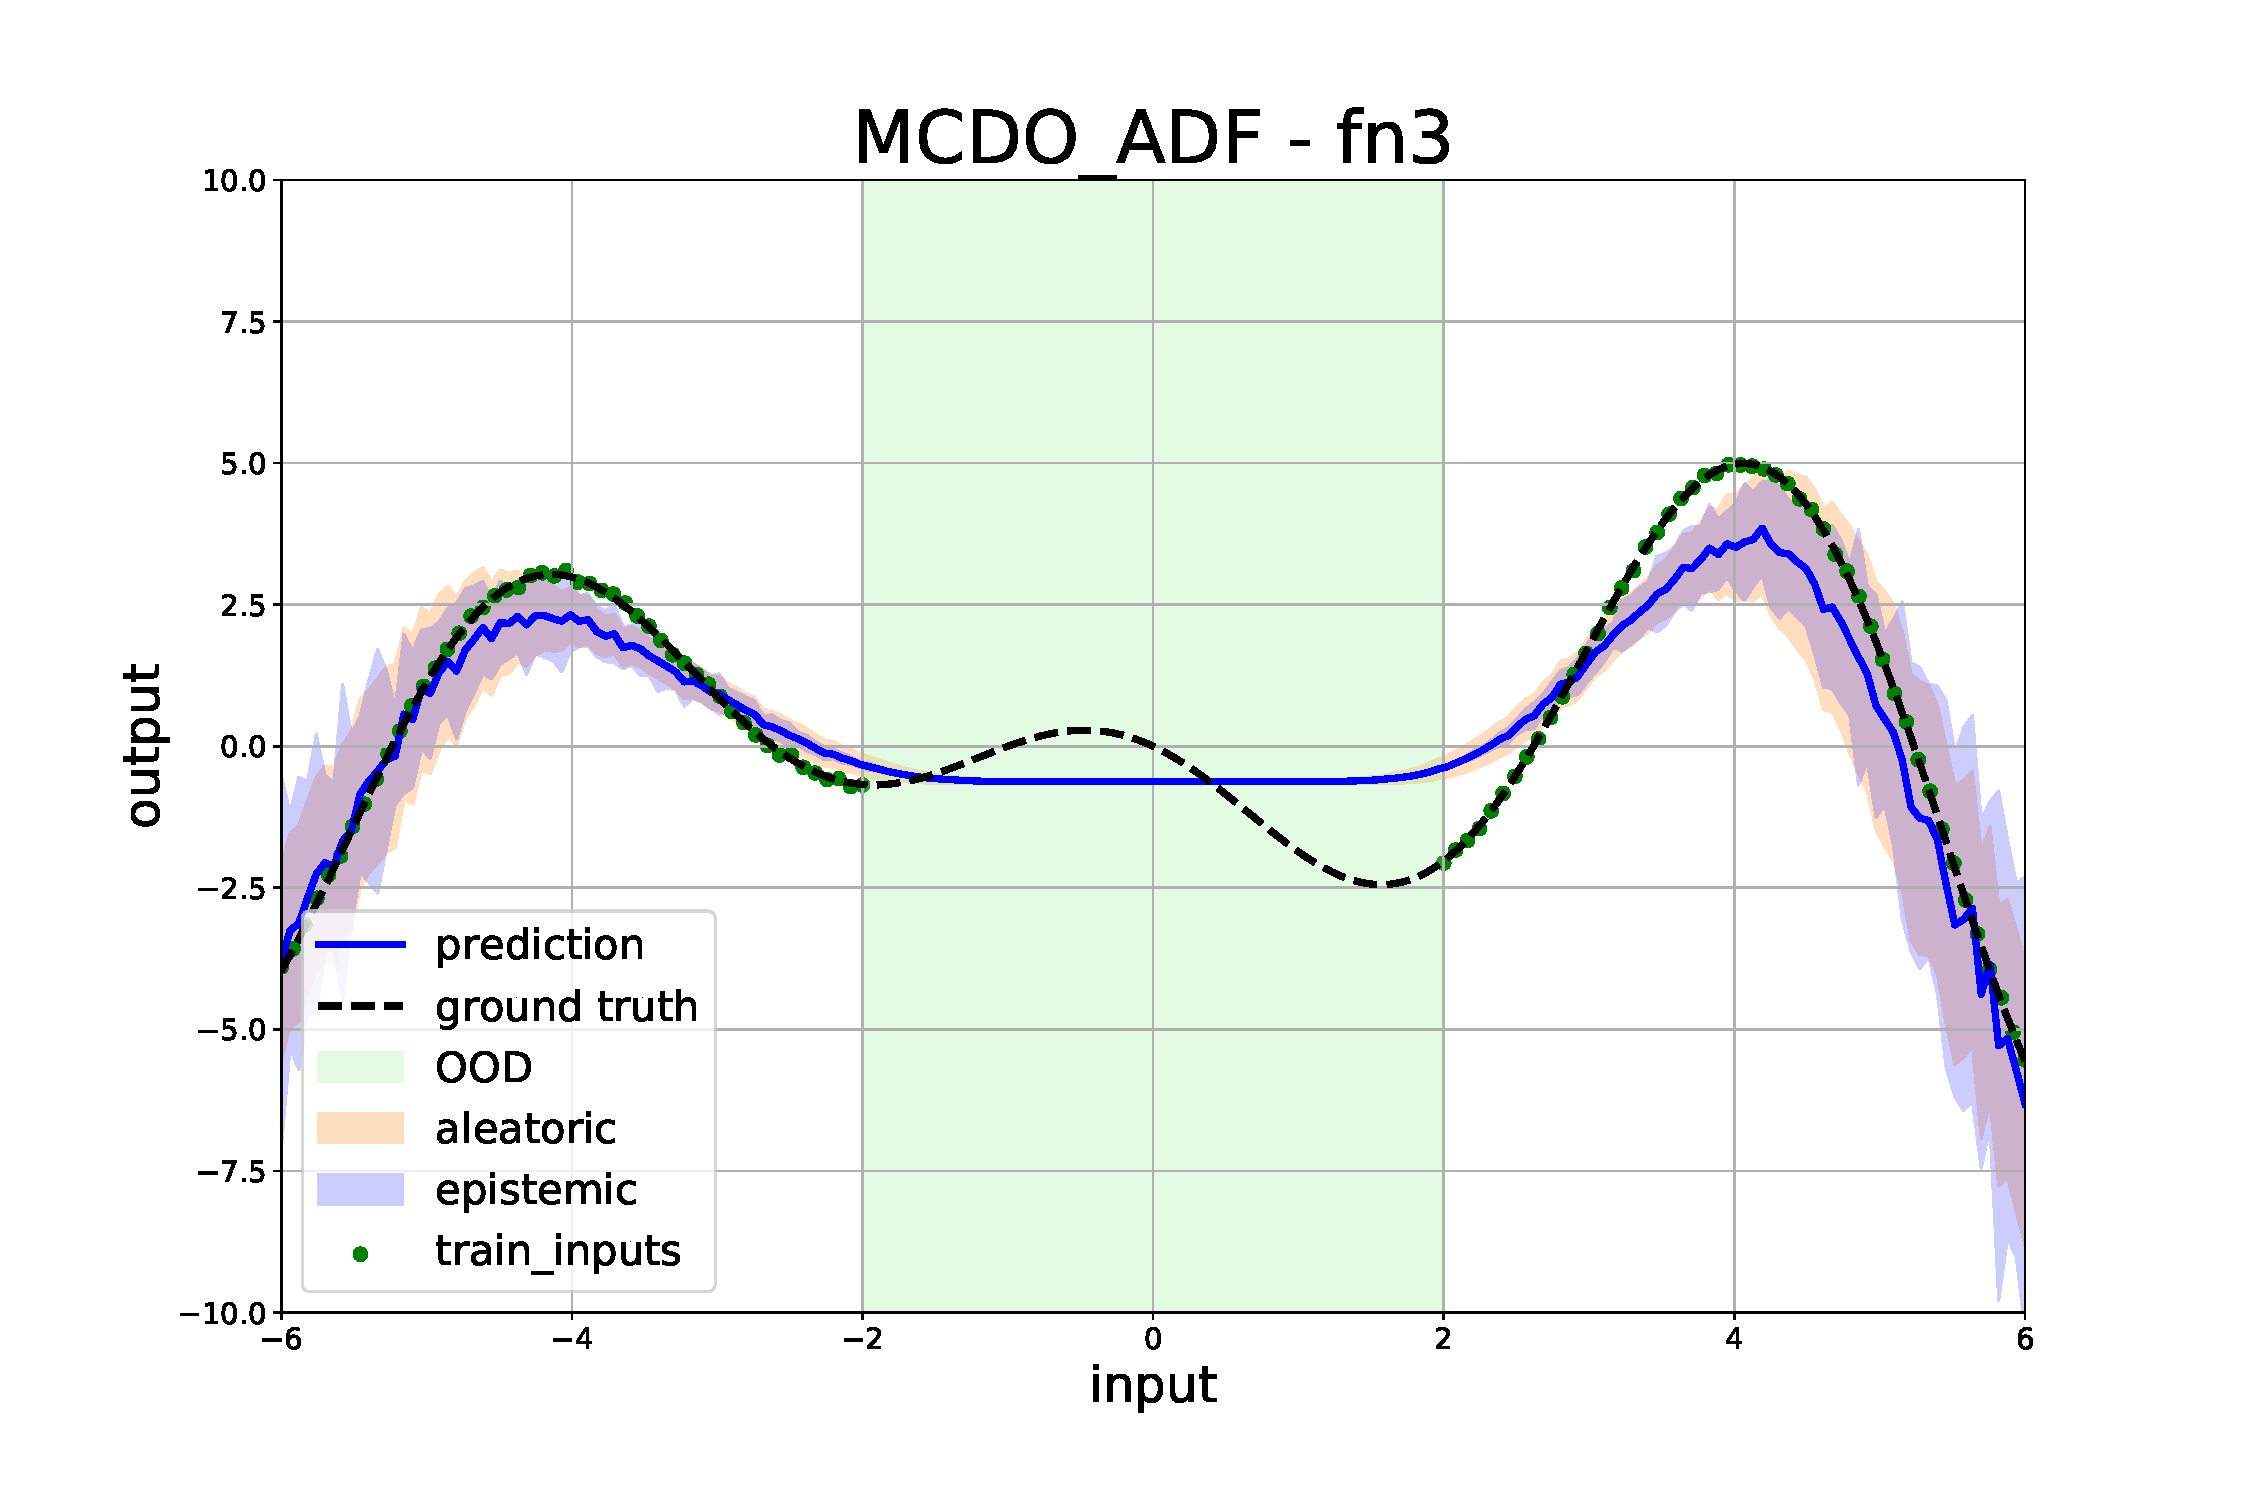
\includegraphics[width=\textwidth]{toy_dataset/mcdo_fn3}
	\caption{$\epsilon=0.06$}
	\label{fig:five over x}
	\end{subfigure}
	\hfill
	\begin{subfigure}[b]{0.4\textwidth}
	\centering
	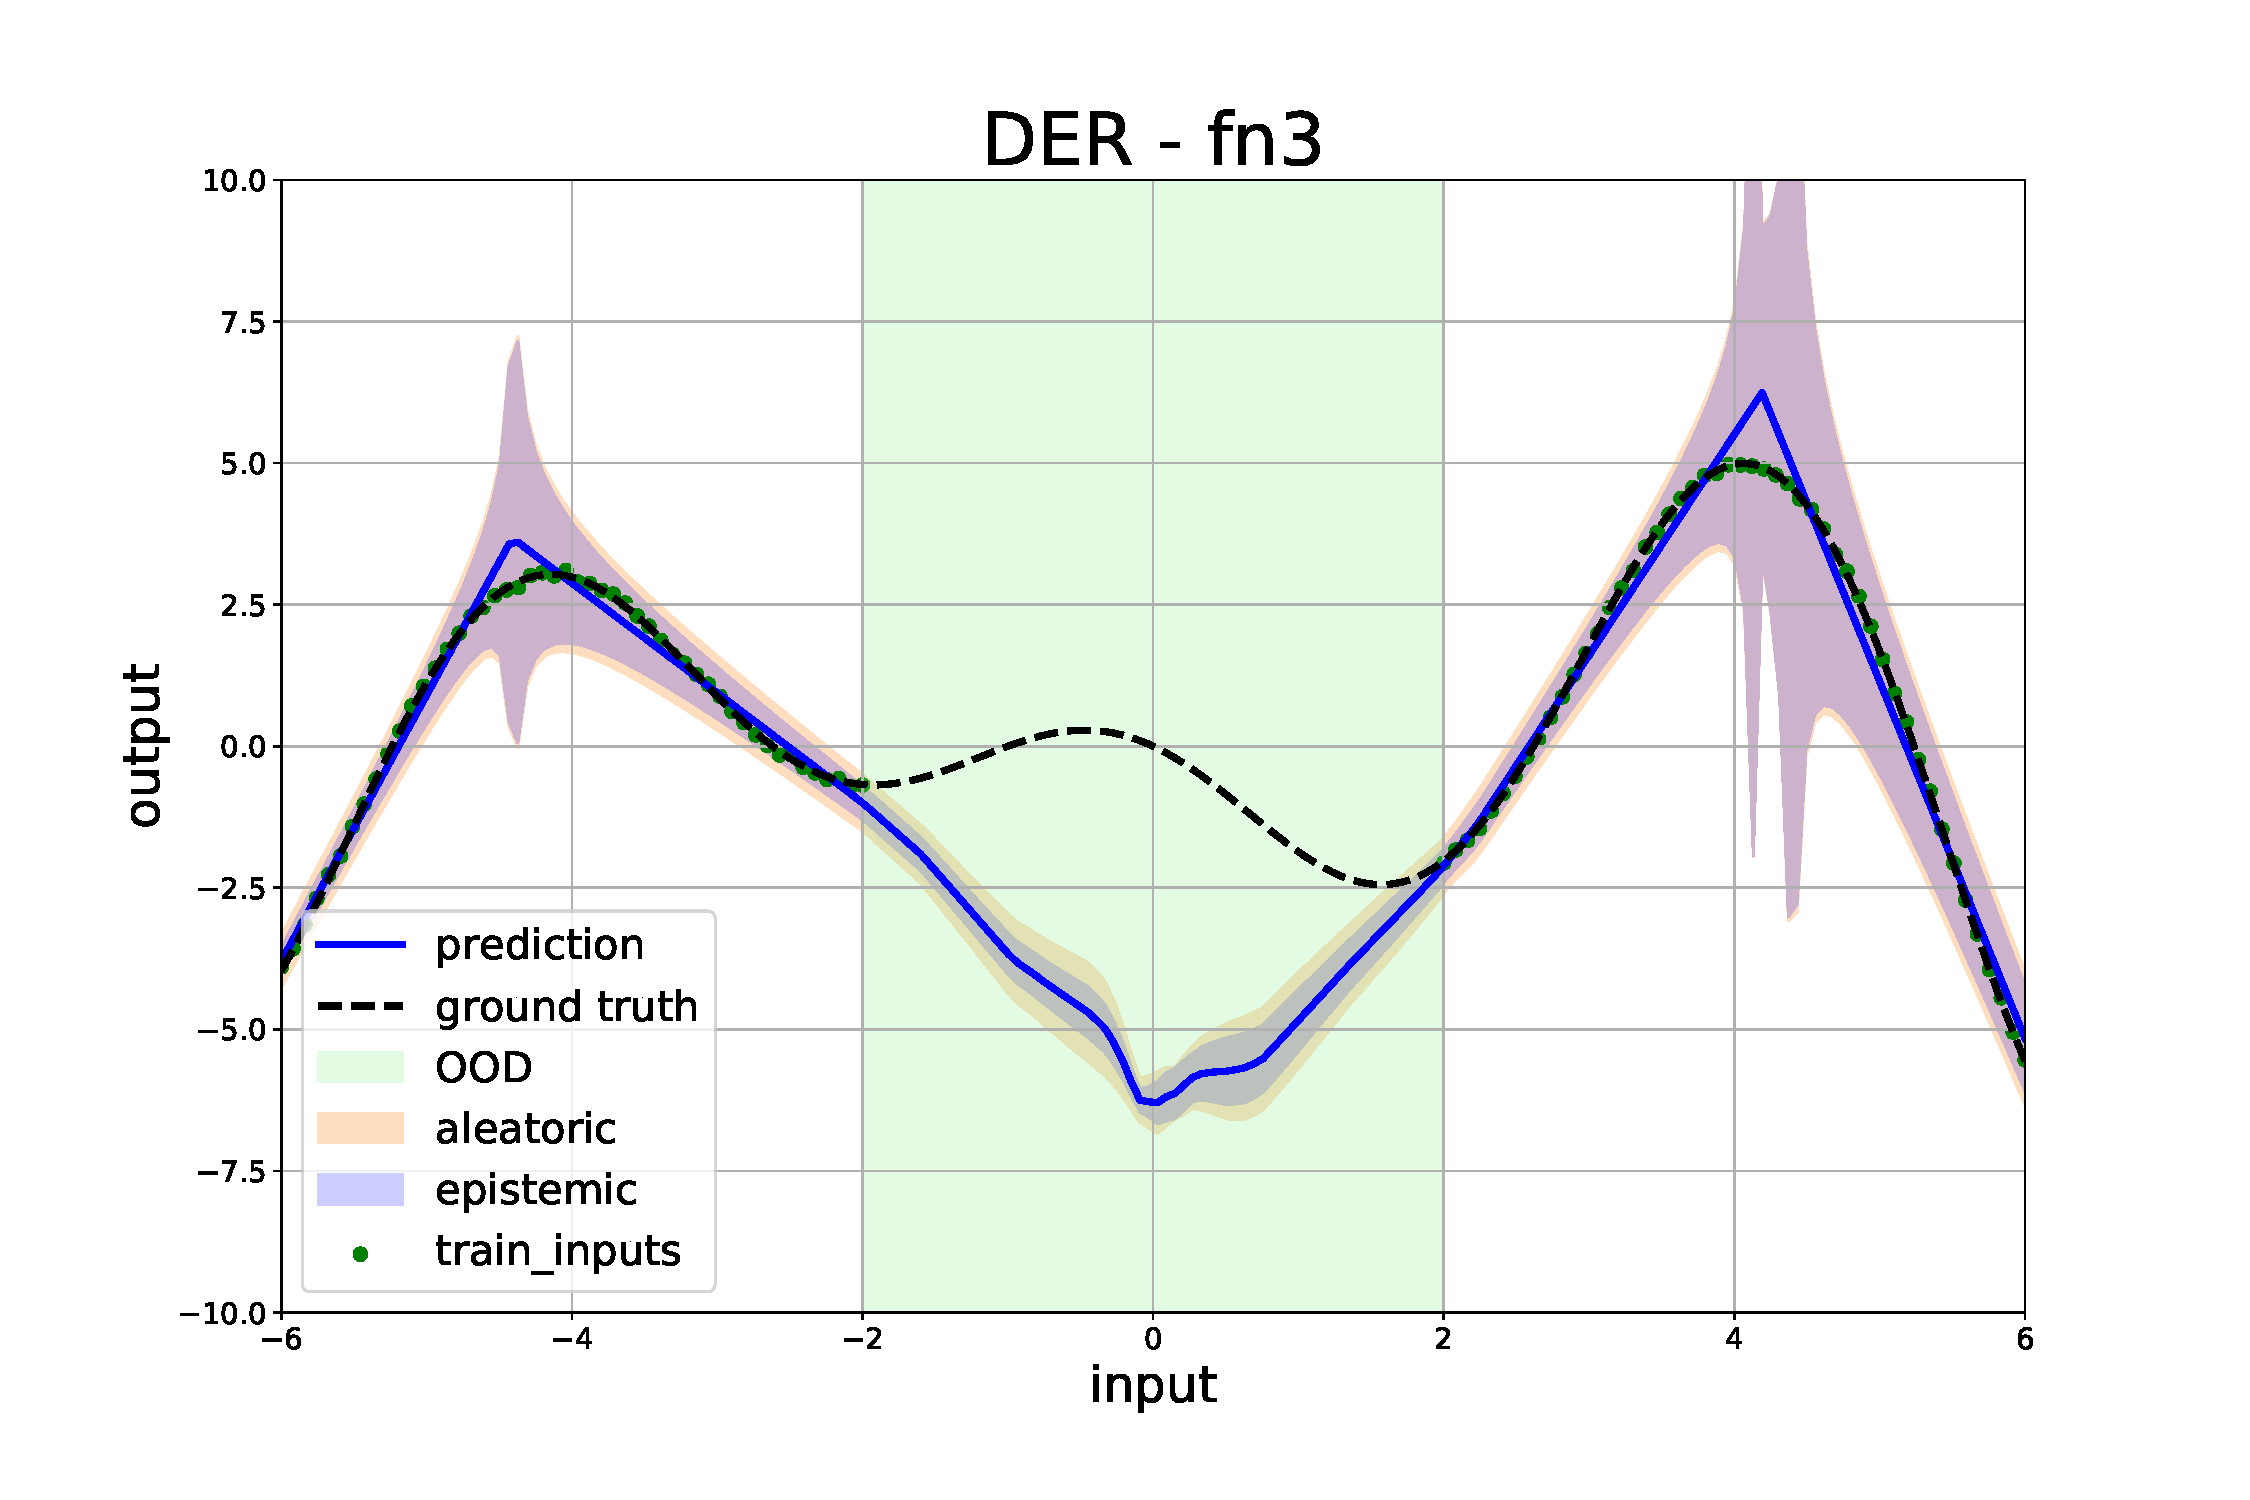
\includegraphics[width=\textwidth]{toy_dataset/der_fn3}
	\caption{$\epsilon=0.06$}
	\label{fig:five over x}
	\end{subfigure}
	\hfill
	\caption{Images depicting increasing levels of Adversarial noise}
	\label{fig_adv_example}
\end{figure}

% Please add the following required packages to your document preamble:
% \usepackage{multirow}
\begin{table}[H]
	\begin{tabular}{|c|c|c|c|c|c|}
		\hline
		\textbf{\begin{tabular}[c]{@{}c@{}}Function\\ y=f(x)\end{tabular}} & \textbf{Metric} & \textbf{\begin{tabular}[c]{@{}c@{}}Homoscedastic\\ GP\end{tabular}} & \textbf{\begin{tabular}[c]{@{}c@{}}Heteroscedastic\\ GP\end{tabular}} & \textbf{Evidential} & \textbf{MCDO\_ADF}                    \\ \hline
		\multirow{3}{*}{$y=\frac{sin(3x)}{3x}$}                            & NLL             & \textbf{-0.82}                                                      & -0.51                                                                 & 0.57                & 2.27                                  \\ \cline{2-6} 
		& RMSE            & \textbf{0.07}                                                       & 0.08                                                                  & 0.40                & 0.39                                  \\ \cline{2-6} 
		& EVA             & \textbf{0.94}                                                       & 0.91                                                                  & -0.29               & -0.43                                 \\ \hline
		\multirow{3}{*}{$y=0.1x^3$}                                        & NLL             & \textbf{-2.44}                                                      & -1.77                                                                 & -0.15               & 1.11                                  \\ \cline{2-6} 
		& RMSE            & \textbf{$\sim$0.00}                                                 & 0.03                                                                  & 0.23                & 0.11                                  \\ \cline{2-6} 
		& EVA             & 0.99                                                                & 0.99                                                                  & \textbf{0.99}       & 0.99                                  \\ \hline
		\multirow{3}{*}{$y=-(1+x+sin(1.2x)$}                               & NLL             & \textbf{-1.02}                                                      & 1.91                                                                  & 6.14                & \textgreater{}\textgreater{}1(182049) \\ \cline{2-6} 
		& RMSE            & 0.61                                                                & \textbf{0.15}                                                         & 2.68                & 0.8                                   \\ \cline{2-6} 
		& EVA             & 0.94                                                                & \textbf{0.99}                                                         & -0.05               & 0.87                                  \\ \hline
	\end{tabular}
\end{table}

\end{document}
